% TODO:
% Вічитка
% прогнать проверку правописания
%
%


\documentclass[12pt]{article}

\usepackage{amsmath,amsthm,amssymb}
\usepackage{mathtext}
\usepackage[T1,T2A]{fontenc}
\usepackage[utf8]{inputenc}
\usepackage[ukrainian]{babel}
\usepackage{listingsutf8}
\usepackage{titling}
\usepackage{multicol}
\usepackage{epigraph}
\usepackage[sorting=none]{biblatex}
\usepackage{tikz}
\usepackage{float}
\usepackage{subfigure}
\usepackage{amsthm}
\usepackage{csquotes}
\usepackage{proof}

\selectlanguage{ukrainian}
\addbibresource{bibl.bib}

\usepackage
[
        a4paper,
        left=3cm,
        right=3cm,
]
{geometry}


\lstset{
    basicstyle=\ttfamily,
    inputencoding=utf8,
    extendedchars=false,
    keepspaces = true,
    language=haskell,
    tabsize=2,
    commentstyle=,
    % keywordstyle=\usefont{T2A}{fcr}{b}{n},
    % backgroundcolor=\color{lightlightgray},
    frame=single,
    tabsize=2,
    captionpos=b,
    caption=\lstname,
    breaklines=true,
    breakatwhitespace=true,
    showstringspaces=false,
    showspaces=false,
    showtabs=false,
    columns=flexible,
    literate={∀}{{$\forall$}}1{λ}{{$\lambda$}}1{∪}{{$\cup$}}1
}
\title{Розподілене конкурентне програмування 
    за допомогою Cloud Haskell}
\author{Микита Юрченко}
\date{Складено \today}

\setlength{\droptitle}{-10em}

\begin{document}

\newtheorem*{definition}{Визначення}
\newtheorem*{theorem}{Теорема}
\newtheorem*{corollary}{Наслідок}
\newtheorem*{axiom}{Аксіома}
\newtheorem*{notation}{Нотація}
\renewenvironment{proof}{{\bfseries Доказ}}

\setlength{\epigraphwidth}{.55\textwidth}

\maketitle

\tableofcontents

\section{Вступ}
%Для чого використовувати і коли застосовувати (клас задач, вимоги до задач)

Cloud Haskell - це EDSL (Embedded Domain-Specific Language) для розробки розподілених відказостійких 
конкурентних\footnote{Традиційно прийнято перекладати concurrency як багатопоточне, або паралельне 
програмування. З точки зору Гаскеля різниця між concurrent та parallel є важливою\cite{marlow}. 
Я вслід за В. Брагілевським перекладаю concurrency як конкурентність\cite{bravit}.} додатків, заснований 
на моделі обміну повідомленнями, подібний Erlang OTP \cite{haskellInCloud}\cite{epsteinThesis} та MPI.\\ 

Сучасні веб-додатки мають обробляти великі обсяги даних, тож виникає потреба не тільки в ефективному 
розподілені роботи між обчислювачами одного комп'ютера, а й між багатьма комп'ютерами, об'єднаними в 
кластер. Надвеликі обчислювальні кластери, які продають свої ресурси користувачам, дістали назву Хмар 
(Cloud).\\

Традиційні підходи до конкурентного програмування на багатоядерних процесорах використовують спільну пам'ять. 
На відміну від них, модель акторів, яку імплементовано в Ерланзі, не дозволяє жодної імпліцитної комунікації 
між процесами. \textit{Абстрагування транспортного рівня від моделі виконання практично стирає принципову 
різницю між локальними та віддаленими обчислювачами}. Можна розробляти програму, використовуючи лише один 
комп'ютер, а потім, доклавши незначни зусилль, необмежено масштабувати її. Цей підхід Д. Армстронг назвав 
у своїй дисертації <<Abstracting out concurrency>>\cite{armstrongThesis}. Таким чином, хоча цей підхід 
цілком сприятливий для програмування одного комп'ютера, його справжня сила розкривається при роботі з 
розподіленими веб-серверами та кластерами для наукових обчислень.\\

Сфера застосування Cloud Haskell дещо ширша, ніж в Ерлангу. Найбільш ефективно буде застосовувати CH для 
розробки алгоритмів, які передбачають великі незалежні обчислювання, наприклад:
\begin{itemize}
\item Великі дані
\item Машинне навчання (нейронні мережі)
\item Високонавантажені веб-додатки
\item Відказостійкі розподілені системи
\item Наукові обчислення
\end{itemize}

Cloud Haskell недоцільно використовувати для наступних задач:
\begin{itemize}
\item Додатки, які потребують сильної оптимізації під конкретне залізо
\item Додатки, які активно взаємодіють з іншими мовами програмування
\item Тісно зчеплені (tight coupling) підзадачі, які вимагають багато синхронізації
\end{itemize}

Деякі переваги Cloud Haskell порівняно з Erlang:
\begin{itemize}
\item Більш продуманий синтаксис
\item Кращі бібліотеки
\item Дозволяє користуватися роздільною пам'яттю на одній машині
\item Типізовані канали
\item Система типів
\item Метапрограмування
\item Користувацька серіалізація
\end{itemize}

На сьогодні в багатьох популярних мовах програмування модель акторів представлено у вигляді портованої 
бібліотеки Scala Akka. Порівняння трьох підходів наведено у таблиці \ref{comparisonTable}.

\begin {table}[H]
\begin{center}
\begin{tabular}{ c|c|c|c } 
              & Erlang OTP  & Scala Akka           & Cloud Haskell            \\
\hline
Реліз         & 1987        & 2009                 & 2012                     \\ 

Версія        & 20.1        & 2.5.6                & 0.7.7                    \\ 

Типізація     & Динамічна   & Дин. примітиви       & Повністю статична        \\ 

Гаряча заміна & Так         & Так                  & Ні                       \\ 

Компіляція    & BEAM VM     & JVM                  & Нативний код             \\ 

Серіалізація  & Автоматична & Автоматична          & Визначається користувачем\\ 
              &             &                      & (або виводиться)         \\ 

Використання  &             &                      &                          \\
примітивів    & Неможливо   & STM                  & MVar, TVar               \\ 
синхронізації &             &                      &                          \\

\end{tabular}
\caption {Порівняння Erlang, Scala та Haskell}
\label{comparisonTable}
\end{center}
\end {table}

\section{Інсталяція}
%Які апаратні засоби та ПЗ потрібно, де його взяти, як встановити, як інтегрувати, наприклад з Visual Studio, якщо це можливо.

\epigraph{My setup = A compiler, emacs, bash, make, an os (I'm not religious here) pencil, paper, coffee, quiet environment, good nights sleep.}{Джо Армстронг}

Реферат було виконано з використанням ОС NixOS (GNU Linux) \cite{nixos}. Стек розробки, який використовує автор, 
є розповсюдженим серед програмістів на Гаскелі, але програмістам на мейнстрімових мовах може здатись незвичним.

\begin{itemize}
\item GNU Emacs 25 (з плагіном haskell-mode)
\item Haskell Stack
\item NixOS 17.03
\item GHC 8.02
\end{itemize}

Засіб є досить високорівневим і не накладає специфічних вимог на апаратне забеспечення. Насправді, його можна 
підняти як на Raspberry Pi \cite{cloudPi}, так й на суперкомп'ютері Altamira \cite{Altamira}. Приклади складено 
автором на його домашньому AMD Phenom II X4 945 3.0 GHz з 4 Gb RAM. У разі потреби, конфігураційні файли автора 
можна знайти у \cite{dotfiles}\\

На сьогодні, єдине, що необхідно для початку роботи з Гаскелем - це Stack.\\

\lstinline{[nik@nixos:~/projects]$ nix-env -iA nixos.haskellPackages.stack}\\

Готовий проект можно завантажити за посиланням \cite{sources}. Кроки, необхідні для самостійного відтворення, 
буде наведено нижче.\\

\lstinline{[nik@nixos:~/projects]$ stack new CloudRef simple}\\

Буде створено проект з такою стуктурою:

\begin{lstlisting}[language=bash, caption={Структура початкового проекту}]
[nik@nixos:~/projects]$ tree CloudRef --charset=ascii
CloudRef
|-- CloudRef.cabal
|-- LICENSE
|-- README.md
|-- Setup.hs
|-- src
|   `-- Main.hs
`-- stack.yaml
\end{lstlisting}

Збудуймо цей проект.

\begin{lstlisting}[language=bash, caption={Будування та запуск проекту}]
[nik@nixos:~/projects/CloudRef]$ stack init
[nik@nixos:~/projects/CloudRef]$ stack build
[nik@nixos:~/projects/CloudRef]$ stack exec CloudRef
\end{lstlisting}

Має вивести до консолі \lstinline{"hello, world"}. Тепер маємо завантажити необхідні бібліотеки. Налаштуємо 
відповідні рядки у файлах \lstinline{stack.yaml} та \lstinline{CloudRef.cabal} згідно до приведених нижче 
лістингів, та перебудуємо проект за допомогою \lstinline{$ stack build}.\\

\begin{lstlisting}[language=bash, caption={stack.yaml}]
...
extra-deps:
- distributed-process-0.7.3
- network-transport-tcp-0.5.1
...
nix:
  enable: true
\end{lstlisting}

Скорегуємо \lstinline{CloudRef.cabal} як показано в наступному лістингу:\\

\begin{lstlisting}[language=bash, caption={CloudRef.cabal}]
...
executable HelloCloud
  hs-source-dirs:      src
  main-is:             HelloCloud.hs
  default-language:    Haskell2010
  build-depends:       base >= 4.7 && < 5
                     , distributed-process == 0.7.3
                     , network-transport == 0.4.4.0
                     , network-transport-inmemory == 0.5.2
\end{lstlisting}

Створимо \lstinline{src/HelloCloud.hs}, який просто виводить до консолі "Hello, Haskell!".\\

\begin{lstlisting}{src/HelloCloud.hs}
import Control.Distributed.Process
import Control.Distributed.Process.Node 
import Control.Concurrent
import Network.Transport
import Network.Transport.InMemory 

main :: IO ()
main = do
  -- Створимо новий транспорт
  t <- liftIO createTransport

  -- Створимо нову локальну ноду
  n <- newLocalNode t initRemoteTable

  -- Запустимо на ній процес
  forkProcess n $ do
    say "Hello, Haskell!"

  -- Чекаємо секунду, аби процес встиг
  liftIO (threadDelay (10^6))

  -- Акуратно закриваємо транспорт
  closeTransport t

\end{lstlisting}

Виконаємо наш приклад за допомогою \lstinline{$ stack build && stack exec HelloCloud}. 
Має вивести до консолі щось, подібне до\\

\begin{lstlisting}[language=bash, caption={Будування та запуск HelloCloud.hs}]
...
[nik@nixos:~/projects/CloudRef]$ stack build && stack exec HelloCloud
Sat Nov 11 14:16:49 UTC 2017 pid://1:8: Hello, Haskell!
\end{lstlisting}

Кожного разу перебудовувати цілий проект, а потім шукати рядки з помилками досить незручно. Автор радить 
усім користуватися плагіном haskell-mode\cite{haskellModeManual} для текстового редактору Emacs\cite{emacs}, 
який можна просто завантажити за допомогою репозиторію MELPA прямо з самого Emacs\cite{haskellModeInstall}. \\

Відкрийте необхідний .hs файл та виконайте \texttt{С-с С-l}. Має відкритися буфер інтерпретатору 
GHCi\cite{ghci}. З нього ви можете запускати функції, визначені та імпортовані в поточному файлі. щоб 
перезавантажити файл, достатньо повторити комбінацію \texttt{С-с С-l}, або набравши \texttt{:r} в інтерпретаторі. \\

Насправді, ви можете користуватися інтерпретатором й без Emacs, прямо з консолі за допомогою 
команди \lstinline{$ stack ghci}. \\

Для профілювання нам стане у нагоді програма ThreadScope. Для її встановлення скористуємося 
\lstinline{$ nix-env -iA nixos.haskellPackages.threadscope}.\\

Знімок робочого оточення автора наведено на рис.\ref{emacs}.\\

\begin{figure}[H]
  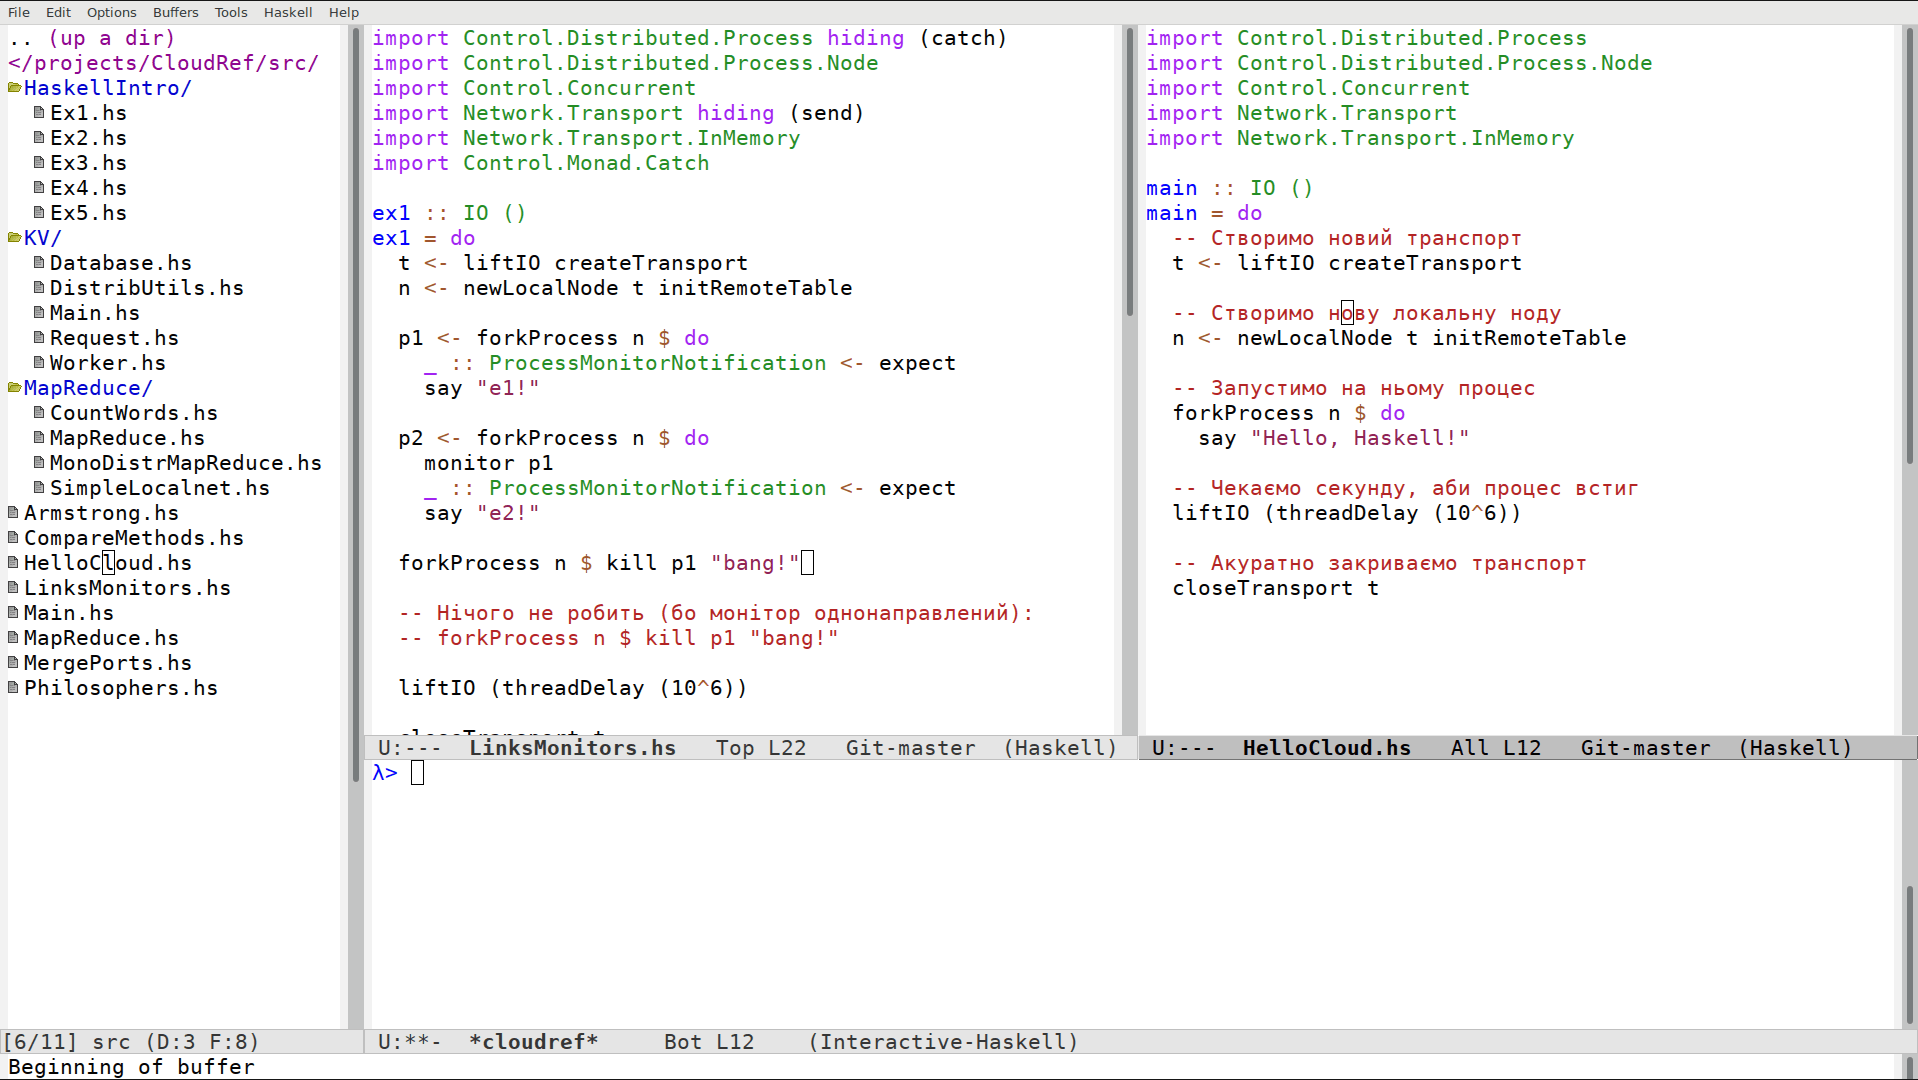
\includegraphics[width=\linewidth]{emacs1.png}
  \centering
  \caption{Робоче оточення}
  \label{emacs}
\end{figure}

Якщо все вийшло, то ми можемо вважати себе повністю готовими до занурення у світ Cloud Haskell.\\

%Загальна теорія (в мови програмування – синтаксис мови, основні конструкції). В разі графічних карт – які 
%типи пам’яті, рекомендації по їх застосуванню

\section{Синтаксис та основні конструкції мови Гаскель}
\epigraph{My prediction is, that in the end, parallel programming will mean functional programming}{Саймон Пейтон-Джонс}

Гаскель - поліморфна компільована чисто функціональна лінива мова програмування з багатою системою типів.\\

Головні властивості:
\begin{enumerate}
\item Вивід типів в стилі Дамаса-Гіндлі-Мілнера
\item Поліморфізм вищих рангів
\item Нестрога семантика, імплементована важким рантаймом на базі STG машини
\item Алгебраїчні типи даних
\end{enumerate}

В цьому рефераті під Haskell ми маємо на увазі GHC Haskell, тобто реалізацію специфікації компілятором 
GHC (Glorious Glasgow Haskell Compiler).\\

На відміну від Java або Rust, абсолютно неможливо людину, яка не має жодного досвіду програмування на 
ML-подібній мові, навчити писати на достатньому для Cloud Haskell рівні, просто виклавши 
<<деякі особливості синтаксису>>, або <<основні інтуїції>>\footnote{З цього  не випливає, що haskell 
є важкою мовою програмування. Його синтаксис є тривіально простим (Див. розділ System FC на стор.\pageref{systemFC}). 
А ось підходи та традиції дійсно неможливо охопити в рамках даного реферату.}.\\


\subsection{Типи та функції}

Всі приклади в цьому розділі не призначені для компіляції. 
Передбачається, що читач буде грати з ними з GHCi. 
Надалі рекомендується виконувати перевірку типів та 
невеликі тести з консолі GHCi, бенчмарки - лише після
повноцінної компіляції.\\

Програмування на Haskell полягає в визначенні типів даних та функцій над ними. Наприклад, визначення типу 
натуральних чисел та їх складання:\\

\begin{lstlisting}{src/HaskellIntro/Ex1.hs}
{-# LANGUAGE GADTs #-}

data N where
  Z :: N
  S :: N -> N

add :: (N, N) -> N
add (a, b) = case b of
  S b' -> S (add (a, b'))
  Z -> a

five = add (S (S Z), (S (S (S Z))))
\end{lstlisting}

Типи визначаються як множини їх значень. Значеннями типа є т.з. конструктори даних, в нашому випадку це Z та S. 
Майте на увазі, що зазвичай використовують скорочений синтаксис вигляду \lstinline{data N = Z | S N}. 
Типи даних є алгебраїчними - | можна розглядати як + (більш точно - як розмічене об'єднання множин), пробіл між 
аргументами конструктору - як * (точніше - як декартів добуток). Тож всі конструюються як суми добутків. 
Алгебраїчні типи є алгебраїчними настільки, що можна навіть брати їхню похідну. Наведемо в якості прикладу 
також визначення класичного АТД "Двійкове дерево": \lstinline{data BTree a = E | Node a (BTree a) (BTree a)}. 
Одним з елементів цього типу буде, наприклад, \lstinline{t1 = Node 2 (Node 1 E E) (Node 3 (Node 4 E E) E)}.

Функції визначаються як рівняння, в яких зазвичай використовують техніку зіставлення зі зразком. Ці рівняння мають 
багато спільного зі звичними математичними рівняннями, наприклад (N, N) можна розглядати як декартів добуток 
множини натуральних чисел з собою. Цей приклад є дещо надмірним - на початку зумисно приведено приклад 
анотації та використання синтаксичного розширення.\\

\subsection{Класи типів}

Можна розглядати класи типів як декотру аналогію інтерфейсу зі світу ООП\footnote{До речі, в мові Idris вони 
так і називаються.}. Нехай до класу типів \lstinline{Summable} входять всі типи, для яких ми визначимо 
операцію складання.\\

\begin{lstlisting}{src/HaskellIntro/Ex3.hs}
class Summable a where
  add :: a -> a -> a
\end{lstlisting}

Визначимо двох представників цього класу типів.\\

\begin{lstlisting}{src/HaskellIntro/Ex3.hs}
instance Summable Int where
  add a b = a + b

instance Summable [a] where
  add xs ys = xs ++ ys
\end{lstlisting}

Продемонструємо використання цієї конструкції. Програмістам на мейнстрімових мовах це має нагадати ad-hoc поліморфізм.\\

\begin{lstlisting}{src/HaskellIntro/Ex3.hs}
main = do
  print (1 `add` 2)
  print $ [1,2,3] `add` [4,5,6]
\end{lstlisting}

Цей приклад видасть помилку \lstinline{Ambiguous type variable}. Це означає, що Гаскель не може підставити 
конкретний тип замість типової змінної. Річ у тім, що операція складання сама визначена у термінах класу 
типів \lstinline{(+) :: Num a => a -> a -> a}. Гаскель підтримує перевантаження літералів. Тож маємо 
підказати компіляторові необхідний монотип:\\

\begin{lstlisting}{src/HaskellIntro/Ex3.hs}
main = do
  print ((1 :: Int) `add` 2)
  print $ [1,2,3] `add` [4,5,6]
\end{lstlisting}

Патерн <<візьми дві а-шки, та зроби з них третю>>, продемонстрований вище, є досить розповсюдженим як в 
програмуванні, так й в алгебрі. Як й усі найважливіші класи типів, його назва прийшла зі світу 
абстрактної алгебри - Моноїд\footnote{Це неправда. Для моноїду необхідний також нейтральний елемент $\epsilon$ (mempty) та умова асоціативності, 
тож це лише магма або полугрупа. Але історично полугрупа не знайшла широкого застосування в Гаскелі.} (Monoid з операцією mappend). 
Інші важливі класи типів - Functor, Monad, Applicative - теж мають алгебраїчне\footnote{Точніше - теоретико-категорне} 
походження.\\

З точки зору Haskell Core (див. стор. \ref{systemFC}), немає жодних Constraint-ів. Розглянемо два найбільш вживані функтори\footnote{Функтор можна розглядати як запаковане значення, всередину якого можна закинути функцію та застосувати її до значення, яке там ховається. В паралельному програмуванні одним з найважливіших функторів є Футура (Async). Також, кожна монада є (аплікативним) функтором.} - список та \lstinline{Maybe a = Just a | Nothing}.

\begin{lstlisting}{src/HaskellIntro/Ex5.hs}
-- * -> * - кайнд = тип типу
class Functor (f :: * -> *) where
  (<$>) :: (a -> b) -> f a -> f b

-- Правоасоціативний оператор пріоритету 6
infixr 6 <$>

instance Functor [] where
  f <$> [] = []
  f <$> (x:xs) = f x : f <$> xs

instance Functor Maybe where
  f <$> Nothing = Nothing
  f <$> Just x  = Just (f x)
\end{lstlisting}

Розцукровування виконується таким чином:

\begin{lstlisting}{src/HaskellIntro/Ex5.hs}
data FunctorI f = FunctorI {
  fmap :: forall a b . (a -> b) -> f a -> f b }

_ListFunctorI :: FunctorI []
_ListFunctorI  = FunctorI { fmap = helper }
  where helper f []     = []
        helper f (x:xs) = f x : helper f xs

_MaybeFunctorI :: FunctorI Maybe
_MaybeFunctorI  = FunctorI { fmap = helper }
  where helper f Nothing  = Nothing
        helper f (Just x) = Just (f x)

-- λ> (+1) <$> [1..100] == fmap _ListFunctorI (+1) [1..100]
-- True
\end{lstlisting}

Тепер товсті стрілки замінюються звичайними, але треба 
передавати додатковий аргумент (реально передається 
словник instance-ів).

\begin{lstlisting}{src/HaskellIntro/Ex5.hs}
(<$$>) :: Functor f => (a -> a) -> f a -> f a
f <$$> box = f <$> f <$> box

fmap2 :: FunctorI f -> (a -> a) -> f a -> f a
fmap2 i f x = fmap' f (fmap' f x)
  where fmap' = fmap i

-- λ> (+1) <$$> [1..100] == fmap2 _ListFunctorI (+1) [1..100]
-- True
\end{lstlisting}

Більш детально про компіляцію класів типів можна
почитати у\cite{scrapClasses}.

\subsection{Монади}

\epigraph{Chaque monade exprime donc le monde entier, mais obscurément, confusément, puisqu’elle est finie, et le monde, infini.}{Жиль Дельоз}

{\let\relax\footnotetext{Епіграф: Таким чином, кожна монада виражає весь світ, але незрозуміло, плутано, оскільки вона є скінченною, а світ є нескінченним}}

Користуючись теорією категорій, визначити монаду тривіально просто (моноїд в категорії ендофункторів над декартово замкненою категорією Hask, де об'єкти - типи, морфізми - функції), але з очевидних причин нам доведеться обмежитися інтуїтивним описом їх практичного застосування з т.з. Haskell.
Тут автор докладає до себе надлюдське зусилля, й втримується від виробництва чергового <<туторіала про монади>> й обмежується наведенням основних визначень стандартної бібліотеки.\\



\begin{lstlisting}{src/HaskellIntro/Ex4.hs}
class Monad m where
  (>>=) :: m a -> (a -> m b) -> m b
  return :: a -> m a

(>>) a b = a >>= \_ -> b
\end{lstlisting}

В подальшому буде наведено багато монадичного коду, записаного за допомогою
do-нотації. 20 років тому, коли Haskell ще активно проектувався, постало
питання про обчислення з ефектами. Пропонувалися\cite{lazyClass} різні
конструкції - засновані на продовженнях, функції, які повертають Unit, та
ін. Але найбільш цікавий варіант запропонував Пилип Вадлер - монади. З
філософської точки зору\cite{deleuze}, все, що потрапляє до монади,
залишається навічно в ній. Для дотримання 
чистоти мови код з зовнішніми ефектами (напр, виведення до консолі)
відокремлено від чистого коду 
шляхом загортання його до монади IO. Неможливо витягнути значення з зовнішнього світу, але можна передати туди наше обчислення. Наприклад, зчитування імені з консолі та привітання:\\

\begin{lstlisting}{src/HaskellIntro/Ex2.hs}
main :: IO ()
main = do
  putStrLn "Insert your name:"
  name <- getLine
  putStrLn ("Hello, " ++ name ++ "!")
\end{lstlisting}

Зауважте, що це не є вбудованим <<синтаксичним Бантустаном>>, в якому мова перестає бути чистою - 
насправді, цей код розцукровується у щось, подібне:\\

\begin{lstlisting}{src/HaskellIntro/Ex2.hs}
main2 = putStrLn "Insert your name:"
  >> getLine
  >>= \name ->
        putStrLn ("Hello, " ++ name ++ "!")
\end{lstlisting}

У спрощеному вигляді монаду IO можна представити як монотип монади State. Монада State слугує для розробки послідовних програм зі змінним станом. Має 3 основні операції: \lstinline{get :: State s a}, \lstinline{put :: s -> State s ()} та \lstinline{evalState :: State s a -> s -> a}, тобто \lstinline{type IO a = State RealWorld a}. 

\begin{lstlisting}{src/HaskellIntro/Ex4.hs}
newtype State s a = State { 
  runState :: s -> (a, s) }

get :: State s s
get = State $ \st -> (st, st)

put :: s -> State s ()
put newState = State $ \_ -> ((), newState)

instance Monad (State s) where
  return x = State (\s -> (x, s))
  p >>= k = q where
    p' = runState p 
    k' = runState . k
    q' s0 = (y, s2) where
        (x, s1) = p' s0
        (y, s2) = k' x s1
    q = State q'

data RealWorld = RealWorld

type IO a = State RealWorld a

ex1 :: State (Int, Int) Int
ex1 =
  put (1,2)
  >> get
  >>= (\(a,b) -> return a)
\end{lstlisting}

В подальшому матеріал буде викладено виходячи з того, що читач знайомий з синтаксисом Гаскеля, його основними 
розширеннями, стандартними алгебраїчними конструкціями (напр. монадою), та має в цілому достатній рівень 
експертизи з Haskell.\\


\section{Основи Cloud Haskell}

\subsection{Обмін повідомленнями}

\begin{itemize}
    \item \lstinline{send :: Binary a => ProcessId -> a -> Process ()} - надсилає повідомлення процесові. Не блокується, не викидає жодних виключень.
    \item \lstinline{expect :: forall a. Binary a => Process a} - заблокувати процес, доки черга повідомлень залишається пустою.
    \item \lstinline{expectTimeout :: forall a. Binary a => Int -> Process (Maybe a)} - аналогічно \lstinline{expect}, але деблокується після n мілісекунд.
    \item \lstinline{receiveWait :: [Match b] -> Process b} - аналог ерлангівського receive. Використовується як \lstinline{r <- receiveWait [ match (\m :: T -> r1), ... ]}
    \item \lstinline{receiveTimeout :: Int -> [Match b] -> Process b} - аналог ерлангівського receive after з затримкою n мілісекунд. 
    
\end{itemize}


\subsection{Процеси та ноди, комунікація між ними.}

\begin{itemize}
    \item \lstinline{spawn :: NodeId -> Closure (Process ()) -> Process ProcessId} - запускає серіалізоване замикання на вказаній ноді.
    \item \lstinline{exit :: Binary a => ProcessId -> a -> Process ()} - делікатно (дає можливість вирішувати власну долю) завершити вказаний процес, кинувши \lstinline{ProcessExitException} зі вказаною причиною. 
    \item \lstinline{kill :: ProcessId -> String -> Process ()} - насильно завершити вказаний процес.
    \item \lstinline{catchExit :: Binary a => Process b -> (ProcessId -> a -> Process b) -> Process b} - навішує заданий гендлер відловлювання конкретного типу \lstinline{ProcessExitException}-ів (другий аргумент) на заданий процес.
    \item \lstinline{catchesExit :: Process b -> [ProcessId -> Message -> Process (Maybe b)] -> Process b} - версія \lstinline{catchExit} для багатьох гендлерів одразу.
    \item \lstinline{die :: Binary a => a -> Process b} - \lstinline{exit} з поточного процесу
    \item \lstinline{terminate :: Process a} - негайно завершити поточний процес
\end{itemize}

\subsection{Лінки та монітори, обробка збоїв}

\begin{itemize}
    \item \lstinline{(un)link :: ProcessId -> Process ()} - лінкування до процесу
    \item \lstinline{(un)linkNode :: NodeId -> Process ()} - лінкування до ноди
    \item \lstinline{(un)linkPort :: SendPort a -> Process ()} - лінкування до порту
\end{itemize}

Зауважте, що \lstinline{unlink*} функції є синхронними в тому сенсі, що гарантується неможливість передачі виключення.

\begin{itemize}
    \item \lstinline{monitor :: ProcessId -> Process MonitorRef} - замоніторити процес
    \item \lstinline{monitorNode :: NodeId -> Process MonitorRef} - замоніторити ноду
    \item \lstinline{monitorPort :: forall a. Binary a => SendPort a -> Process MonitorRef} - замоніторити порт
    \item \lstinline{unmonitor :: MonitorRef -> Process ()} - є асинхронною в сенсі, зазначеному вище
\end{itemize}

Якщо процес А замоніторив процес Б, то коли процес Б вмре, або від'єднається, то процес А отримає \lstinline{ProcessMonitorNotification}. Можна мати довільну кількість моніторів $А \longrightarrow Б$.\\

Якщо процес А прилінкувався до процесу Б, то коли процес Б вмре, або від'єднається, то в процесі А буде викинуто виключення. Неможливо мати 2 лінки $А \longrightarrow Б$. Лінки реалізовано за допомогою моніторів\\

На відміну від ерлангу, монітори та лінки є однонаправленими. Розглянемо наступні 2 приклади використання моніторів та лінків відповідно.\\

\begin{lstlisting}{src/LinksMonitors.hs.hs}
ex1 :: IO ()
ex1 = do
  t <- liftIO createTransport
  n <- newLocalNode t initRemoteTable
  
  p1 <- forkProcess n $ do
    _ :: ProcessMonitorNotification <- expect
    say "e1!"
  
  p2 <- forkProcess n $ do
    monitor p1
    _ :: ProcessMonitorNotification <- expect
    say "e2!"

  forkProcess n $ kill p1 "bang!"
  
  -- Нічого не робить бо монітор однонаправлений:
  -- forkProcess n $ kill p2 "bang!"
  
  liftIO (threadDelay (10^6))
  
  closeTransport t

-- ghci:
-- λ> ex1
-- Wed Nov 22 13:41:54 UTC 2017 pid://1:9: e2!
\end{lstlisting}

\begin{lstlisting}{src/LinksMonitors.hs.hs}
ex2 :: IO ()
ex2 = do
  t <- liftIO createTransport
  n <- newLocalNode t initRemoteTable

  let h (e::SomeException) =
        liftIO $ putStrLn $ "[E] " ++ (show e)
  
  p1 <- forkProcess n $ handle h $ expect >>= say  
  p2 <- forkProcess n $ handle h $ link p1 >> expect >>= say

  forkProcess n $ kill p1 "bang!"

  -- Не вбиває перший процес, бо лінки однонаправлені:
  -- forkProcess n $ do
  --   kill p2 "bang!"
  --   liftIO (threadDelay 1000)
  --   send p1 "I am alive!"
  
  liftIO (threadDelay (10^6))
  
  closeTransport t
  
-- ghci:
-- λ> ex2
-- [E] killed-by=pid://1:10,reason=bang!
-- [E] ProcessLinkException pid://1:8 DiedNormal
\end{lstlisting}



\subsection{Типізовані канали}

\begin{itemize}
    \item \lstinline{newChan :: Binary a => Process (SendPort a, ReceivePort a)} - створити новий канал
    \item \lstinline{sendChan :: Binary a => SendPort a -> a -> Process ()} - надіслати повідомлення по каналу
    \item \lstinline{receiveChan :: Binary a => ReceivePort a -> Process a} - зчитати повідомлення з каналу
    \item \lstinline{receiveChanTimeout :: Binary a => Int -> ReceivePort a -> Process (Maybe a)} - чекати повідомлення з каналу n мікросекунд
    \item \lstinline{mergePortsBiased :: Binary a => [ReceivePort a] -> Process (ReceivePort a)} - Об'єднує приймаючі порти, отримуючи новий порт, на який будуть приходити повідомленні я усіх переданих. При цьому, черга повідомлень перевіряється згідно списку.
    \item \lstinline{mergePortsRR :: Binary a => [ReceivePort a] -> Process (ReceivePort a)} - аналогічно mergePortsBiased, але після кожного зчитування відбувається зсув вліво, в результаті перший порт стає останнім
\end{itemize}

Важливо відмітити таку особливість: SendPort можна передавати іншим нодам у повідомленнях, бо він є серіалізовним (тобто є екземпляром класу типів Binary, про який буде наступний підрозділ). ReceivePort є закріпленим, його не можна передавати. Це дуже важливо і зроблено навмисно для спрощення розрахунку cost model.\\

Проілюструємо використання цих функцій.

\begin{lstlisting}{src/MergePorts.hs.hs}
main :: IO ()
main = do
  t <- liftIO createTransport
  n <- newLocalNode t initRemoteTable

  forkProcess n $ do
    (f1, t1) <- newChan
    (f2, t2) <- newChan

    sendChan f1 "m1"
    sendChan f2 "m2"

    receiveChan t1 >>= say
    receiveChan t2 >>= say

    t3 <- mergePortsBiased [t1, t2]
    -- t3 <- mergePortsRR [t1, t2]

    sendChan f2 "m3"
    sendChan f1 "m4"
    sendChan f1 "m5"

    -- RR:     m4 -> m3 -> m5
    -- Biased: m4 -> m5 -> m3
    
    receiveChan t3 >>= say
    receiveChan t3 >>= say
    receiveChan t3 >>= say

  liftIO (threadDelay (10^6))
  closeTransport t

\end{lstlisting}

\subsection{Клас типів Binary. Серіалізація замикань}

Клас Binary a визначає 2 базові операції
\footnote{Якщо подивитись вихідні коди, то там буде
\lstinline| class Binary t where put :: t -> Put; get :: Get t |
, де \lstinline|Put Get| - деякі монади. Ця більш узагальнена форма ніяк 
не конфліктує з нашим простим визначенням зі старої версії.}
\lstinline{encode :: a -> ByteString} та \lstinline{decode :: ByteString -> a} 
такі, що $\forall \mathtt{x} . \mathtt{decode (encode \ x)} = \mathtt{x}$\\

Таким чином, користувач має сам визначити, як йому серіалізовувати той чи інший тип.
Для вбудованих типів цей клас вже визначено. Реалізації автоматично наслідуються. 
Більш того, існує дієвий механізм автоматичного виводу екземплярів цього типу.
Нехай користувач визначив тип \lstinline{data T a = E | N a (T a) (T a)}.
Тоді можна доповнити до \lstinline{data T a = E | N a (T a) (T a) deriving (Typeable, Generic)}, а потім \lstinline{instance Binary a => Binary (T a)}. Також необхідно ввімкнути розширення DeriveGeneric. В результаті, наприклад, \lstinline{encode (N 'a' (N 'b' E (N 'd' E E)) (N 'c' E E)) = \SOHa\SOHb \NUL\SOHd \NUL\NUL \SOHc\NUL \NUL}. Цей приклад демонструє корисність користувацької сериіалізації - ці ж самі двійкові дерева можна було закодувати більш економно кодами Прюфера, чи якось інакше.\\

Виникає питання - як нам передавати функції між процесами? В Ерланзі, завдяки віртуальній машині, все 
є серіалізовним за замовчуванням, в тому числі й функції. Компілятор Haskell не надає подібних можливостей. 
Більш того, цей підхід може викликати певні складнощі. Що таке вільні змінні? Вони самі можуть бути 
функціями, тоді оточення цих функцій теж треба додати до повідомлення (власне, цьому це й називається 
замиканням). Програміст може випадково передати величезне повідомлення лише тому, що вільною змінною 
деякої невеликою функції є, наприклад, база даних. В лінивій мові все стає ще важчим через наявність 
санків.\\

З цього випливає, що має сенс обмежити функції, які можна передавати. Давайте спробуємо зайти з іншого 
боку - які функції ми точно можемо передати? Чи можемо ми передати, наприклад, \lstinline{(+)}? Звісно, 
що так - ця функція завжди доступна в стандартній бібліотеці. Чи можемо ми передати замкнутий терм, до якого не входить жодна вільна змінна?\\

Якщо один й тий самий бінарник виконується на іншому кінці, то ми 
можемо просто передати статичний вказівник на цей код. Оригінальна ідея, запропонована в \cite{haskellInCloud}, полягає в введенні на рівні компілятору конструктору типів \lstinline{Static a}. Головне, що необхідно знати про статичні значення - це те, що вони є серіалізовними. Правила типізації для цих значень наведено в рис. \ref{fractions},  де $\Gamma$ - множина зв'язок змінних та типів, для яких відомо, що вони є або не є S-зв'язаними.

Змінна є S-зв'язаною (S-bounded), 
якщо та тільки якщо всі вільні змінні в ній оголошено на верхньому рівні поточного модуля.\\ 

Змінна є D-зв'язаною якщо і тільки якщо вона не є S-зв'язаною.\\

Терм $\mathtt{static} \  e$ має тип $\mathtt{Static} \ \tau$ в тому і тільки в тому випадку, коли всі вільні змінні $e$ є S-зв'язаними.\\

\begin{figure}[h]
\centering

$\Gamma ::= \overline{x :_\delta \sigma}
\quad\text{(Контекст)}$\\
\vspace{2em}
$\delta ::= S | D
\quad\text{(Помітка зв'язування)}$\\
\vspace{2em}
$\Gamma \downarrow \ = \ \{x :_s \sigma \:|\: x :_s \sigma \in \Gamma\} \quad \text{(Фільтрування S-зв'язаних)}$\\
\vspace{2em}
$\infer[\quad \text{(Введення \texttt{static})}]{\Gamma \ \vdash \  \mathtt{static} \  e : \mathtt{Static} \  \tau }{\Gamma \downarrow \ \ \vdash\  e : \tau}$\\
\vspace{2em}
$\infer[\quad \text{(Видалення \texttt{static})}]{\Gamma \ \vdash \ \mathtt{unstatic} \ e : \tau}{\Gamma \ \vdash \ e : \mathtt{Static} \ \tau}$ \\

\caption{Правила типізації для static}
\label{fractions}
\end{figure}

Тепер ми можемо записати \lstinline{MkClosure :: Static (e -> a) -> e -> Closure a}. Але де зв'язано змінну e? Вона є екзистенційно квантифікованою, тобто можемо записати щось подібне до \lstinline{[MkClosure (static (`mod` 2)) 42, MkClosure (static ord) '7'] :: [Closure Int]}. Обидві функції захоплюють різний тип e.

Спробуємо поліпшити ситуацію, додавши обмеження на тип e - він має бути серіалізовним \lstinline{MkClosure :: Binary e => Static (e -> a) -> e -> Closure a}. Але навіть для такого типу не буде захоплюватися конкретний тип e, тож десеріалізація неможлива. Можна було б піти далі, передаючи якось це значення типової змінної. Але давайте згадаємо, що ми взагалі знаємо про клас Binary? Всі серіалізовні значення є взаємно відповідними до ByteString.   Тож на щастя існує просте рішення - використовувати в замість e простий тип ByteString.

Для пошуку необхідних функцій генерується словник, в якому ключами є строки, а remotable функції цього модуля - значеннями. 
Щоб не змушувати користувача додавати кожного разу ці функції вручну, розробники Cloud Haskell 
скористалися вбудованим засобом метапрограмування Template Haskell. Для того, щоб помітити функцію 
\lstinline{f} для передачі, достатньо під'єднати модуль \lstinline{Control.Distributed.Process.Closure}, 
додати до файлу директиву компілятора \lstinline|{-# LANGUAGE TemplateHaskell #-}|, та дописати після 
оголошення функції \lstinline{$(remotable ['f])}.

Існують підходи й для серіалізації поліморфних функцій.\\

\subsection{Інші можливості}

\subsubsection*{Unsafe функції}
Unsafe примітиви дублюють основні функції. Якщо звичайні функції нормалізують повідомлення перед пересиланням, 
то їхні unsafe аналоги дозволяють передавати вказівник в межах локальної ноди. Можна використовувати тільки 
за умови повної впевненості у власному коді.\\

\subsubsection*{Мережеві можливості}
Мережевий рівень абстраговано від реалізації. В подальших прикладах будуть використовуватися або InMemory бекенд, або SimpleLocalnet. 
Також існує TCP, Azure та CCI бекенд.\\



\section{Модель акторів}

\epigraph{Oh, yes, this is very $\pi$-calculus stuff!}{Саймон Пейтон-Джонс\cite{cloudSLPJ}}

У статті\cite{cloudSemantics} побудовано математичну\footnote{Unified Semantics, запропонована Свенсоном\cite{svensson}} семантику (деякої підмножини) примітивів Cloud Haskell.\\

\subsection{Що таке актор}

На жаль, на відміну від $\lambda$-числення, точне та відносно повне математичне викладення моделі акторів неможливе без важкого використання теорії доменів, операційної семантики, та ін. Насправді, це типова ситуація для практико-орієнтовних теоретичних побудувань. Тож залишається лише розважати читача неформальним викладом, заснованим на оглядовій статті від автора\cite{hewitt} та на відео\cite{actorsVideo} з його участю.\\

\textbf{Актор} має три функції.
\begin{enumerate}
    \item Обробляє інформацію
    \item Зберігає інформацію
    \item Спілкується напряму з іншими акторами
\end{enumerate}

\textbf{Аксіоми}. Коли актор отримує повідомлення, він може конкурентно:
\begin{enumerate}
    \item надіслати повідомлення іншому акторові (в тому числі самому собі)
    \item створити нових акторів
    \item визначити, як він буде обробляти наступне повідомлення\footnote{Найбільш туманний пункт. 
    Фактично, саме так актор виконує корисні обчислення. Наприклад, якщо актор "Рахунок клієнта N", який зберігає стан "5 доларів", отримує повідомлення "збільшити рахунок на 5 доларів", то якщо наступне повідомлення спитає його про стан балансу, то він відповість "11 доларів".}
\end{enumerate}

Порівняно з популярними імплементаціями (в т.ч. CH), оригінальна модель акторів є більш легковісною. Вона не передбачає:
\begin{enumerate}
    \item Каналів. Всі актори спілкуються безпосередньо один з одним. Втім, канал може бути імплементовано як актор. Це відрізняє модель акторів від іншої популярної моделі процесів, що спілкуються - $\pi$-числення (Про ці відмінності буде більш детально сказано нижче). 
    \item Черги повідомлень (поштової скрині). Актор обробляє лише одне повідомлення. Тож відправник має самостійно смикати адресу призначення, доки не дочекається відповіді. Г'юїтт наголошує на тому, що зі стверджень <<все є актором>> та <<кожен актор має поштову скриню>> випливає, що поштова скриня теж має бути актором. В поштової скрині теж має бути поштова скриня, down to the Rabbit Hole.
    \item Детермінований порядок повідомлень. Якщо актор $\mathcal{A}_1$ надсилає акторові $\mathcal{A}_2$ спочатку повідомлення $m_1$ а потім повідомлення $m_2$, то актор може отримати їх у будь-якому порядку. 
\end{enumerate}

Таким чином, модель акторів є, з одного боку, загальною моделлю обчисленнь (в одному ряді з $\lambda$-численням, машиною Тюрінга, продукціями Поста, рекурсивними функціями Кліні, алгорифмами Маркова, комбінаторами Шенфінкеля, та ін.), а з другого боку - моделлю паралельних обчислень (порівняну з $\pi$-численням, CCS, CSP, мережами Петрі, та ін.).\\

Порівняно з численнями процесів ($\pi$-численням, CCS, CSP), модель акторів не вимагає каналів (але легко може їх імплементувати). Мілнер та ін. ввели канали як примітиви, щоб отримати красиві рівняння. На практиці, якщо двоє намагаються взяти щось з виходу каналу, це вимагає досить складного механізму (two-phased commit), який суттєво збільшує оверхед.\\

Мережі Петрі моделюють потік управління, але не моделюють потік даних.\\

Згідно Г'юїтові, модель акторів не зводиться до недетермінованої машини Тюрінга. Г'юїтт особливо наголошує на незводимості індетермінізму до недетермінізму. Недетермінізм - це те, що ви отримаєте, підкинувши монетку. Індетермінізм виникає в умовах реального світу, наприклад, коли один сервер надсилає іншому два повідомлення по двох різних каналах.\\

\subsection{Індукція по акторах}

\epigraph{Вот Павел Сергеевич, ну известный наш академик, Александров, он никогда не летает на самолете. А вы знаете почему? Он не знает доказательства теоремы Жуковского и поэтому не понимает, как самолет держится в воздухе. А я знаю! И не боюсь летать!}
{Борис Миколайович Делоне}


В якості ілюстрації того, що ми все ж таки маємо справу з строгим математичним формалізмом (втім не таким алгебраїчним, як $\pi$-числення), приведемо формальне визначення індукції по акторах зі статті\cite{actorLaws} Г'юїтта та Бейкера 1977 року. Судячи з невеликого огляду автором найбільш частих посиланнь з теми, це є рідкісна \textit{математична} стаття з теорії акторів, яка не потребує робочого знання теорії доменів, денотаційної та операційної семантики та іншої теорії рівня graduate, а використовує лише найпростішу теорію множин та порядків, відому з першого курсу будь-якому студенту-програмістові. \\

\begin{definition}[Акторне обчислення]
є пара $\langle\mathcal{E}, \longrightarrow\rangle$, де $\mathcal{E}$ - множина подій, $\longrightarrow$ - строгий частковий(= транзитивний антирефлексивний) порядок на множині $\mathcal{E}$. 
\end{definition}

\begin{definition}[Передування]
Кажуть, що $E_1$  передує $E_2$ якщо $E_1 \longrightarrow E_2$.
При цьому, $E_2$ є прямим наступником $E_1$.
\end{definition}

\begin{definition}[Конкурентність]
Кажуть, що $E_1$ є конкурентною з $E_2$, якщо невірно, що $E_1 \longrightarrow E_2$ або $E_2 \longrightarrow E_1$.
\end{definition}

\begin{axiom}[Існування начальної події]
Нехай для зручності множина завжди $\mathcal{E}$ має точну нижню грань $E_{\bot}$, яка називається начальною подією.
\end{axiom}

\begin{axiom}[Фінітність]
Для будь-яких $E_1$ та $E_2$, множина $\{E | E_1 \longrightarrow E \longrightarrow E_2\}$ є скінченною.
\end{axiom}

Без аксіоми фінітності індуктивні докази були б неможливі.

\begin{definition}[Прямий попередник]
$E_p$ є прямим попередником $E$ якщо $\nexists E'\in\mathcal{E}. E_p \longrightarrow E' \longrightarrow E$
\end{definition}

\begin{axiom}[Дискретність]
Для будь-якої події, множина її прямих попередників та прямих наступників є цілком визначеною.
\end{axiom}

\begin{corollary}
З попередніх трьох аксіом випливає, що для будь-якого акторного обчислення існує монотонна ін'єкція у множину позитивних натуральних чисел $f: \mathcal{E} \hookrightarrow \mathbb{N}^{+}$
\end{corollary}

Існування такої ін'єкції демонструє, що клас акторних обчисленнь не може розширювати клас обчислювальних функцій, запропонований Черчем.\\

\begin{displayquote}
\textbf{Теза Черча-Тюрінга-Г'юїтта.} \textit{Всі фізично можливі обчислювання можна напряму імплементувати за допомогою акторів.}\\
\end{displayquote}


\textit{Дія} в моделі акторів складається з об'єктів, які називаються \textit{акторами}. Актори надсилають \textit{повідомлення} іншим акторам, які називаються \textit{цілями} цих повідомленнь. Отже, подія E являє собою отримання повідомлення \texttt{message(E)} актором \texttt{target(E)}.

Коли актор \texttt{target(E)} отримує повідомлення \texttt{message(E)}, він, відповідно до деякої програми обчислює новий локальний стан зі старого, та надсилає повідомлення іншим акторам. Про події, в яких отримуються ці повідомлення говорять, що вони є активованими подією E.

\begin{definition}[Підпорядок]
Підпорядком строгого часткового порядку $\langle A, \leq\rangle$ називають строгий частковий порядок $\langle A', \leq'\rangle$, де $\leq'$ - транзитивне замикання підмножини $\leq$.
\end{definition}

\begin{definition}[Відношення активації]
Відношення активації є деяким визначеним підпорядком відношення передування. Інтуїтивно, відношення активації схоплює поняття каузації у фізичному смислі\footnote{Фотони - повідомлення, атоми - актори. Фотон прилітає до цілі - атому. Відбулася подія <<Атом 1 отримав фотон 1>>. Атом переходить до збудженого стану, виділяє новий фотон 2 та повертається до стабільного стану. Про подію <<Атом 2 отримав фотон 2>> ми скажемо, що її було \textit{активовано} першою подією.}.
\end{definition}

\begin{corollary}
Спостереження. Відношення активації формує дерево, коренем якого завжди є $E_{\bot}$.
\end{corollary}

\begin{definition}[Відношення прибуття]
Нехай на множині $\mathcal{E}$ задано відношення еквівалентності $\simeq$ таке, що $E_1 \simeq E_2$ в тому і тільки в тому випадку, коли \texttt{target($E_1$)} = \texttt{target($E_2$)}. 
Тоді кожному з отриманих класів еквівалентності задано лінейний порядок, що є підпорядком відношення передування, і називається відношенням прибуття.
\end{definition}

\begin{definition}[Секція]
Секцією(перерізом) деякої впорядкованої множини $\langle A, \leq\rangle$ відносно деякого $s \in A$, є або $\{x \in A | x \leq s \}$,або сама ця множина.
\end{definition}

\begin{corollary}
Будь-яке відношення прибуття ізоморфно секції $\mathbb{N}$
\end{corollary}

\begin{theorem}[Індукція по порядку передування]
Для будь-якого акторного обчислення $\langle\mathcal{E}, \longrightarrow\rangle$ та властивості Р, якщо виконуються умови
\begin{enumerate}
    \item $P(E_{\bot})$
    \item $\forall E \in \mathcal{E}. P(\mathtt{activator(E)}) \land P(\mathtt{precursor(E)}) \implies P(E)$
\end{enumerate}
то для буль-якої події $E \in \mathcal{E}$ виконується $P(E)$
\end{theorem}

\begin{proof}
Тривіальний за допомогою слабкої індукції за результатом монотонної ін'єкції.
\end{proof}

Докладне та повне викладення багатьох технік формального доказу властивостей акторних программ можна знайти у\cite{yonezawa} .

%(і подальші розділи, якщо необхідно: Приклади використання з додатками у вигляді повних проектів, з порівнянням зі стандартними засобами 
\section{Порівняння зі стандартними засобами}
Складемо функцію \lstinline{primeFactors} для розрахунку простих множників числа. 

\begin{lstlisting}{src/CompareMethods.hs - primeFactors}
factorize :: Integer -> Integer -> [Integer]
factorize _ 1 = [] 
factorize d n 
    | d * d > n = [n]
    | n `mod` d == 0 = d : factorize d (n `div` d)
    | otherwise = factorize (d + 1) n

primeFactors :: Integer -> [Integer]
primeFactors = factorize 2
\end{lstlisting}

Допоміжна функція для розділення списку на декілька рівновеликих підсписків:\\

\begin{lstlisting}{src/CompareMethods.hs - divideList}
divideList :: Int -> [a] -> [[a]]
divideList n xs = divideList' xs
  where m = (length xs `div` n) + 1
        divideList' [] = []
        divideList' xs = take m xs : divideList' (drop m xs)
\end{lstlisting}

В якості важкого завдання, яке можна виконувати паралельно, нехай буде знаходження суми простих 
множників чисел від from включно до to включно.

\begin{lstlisting}{src/CompareMethods.hs - Sequential}
--Послідовне виконання
main0 :: IO ()
main0 = print $ sum $ map (sum . primeFactors) [from..to]
\end{lstlisting}

\begin{lstlisting}{src/CompareMethods.hs - Control.Concurrent}
--Вбудовані засоби конкурентного програмування
main1 :: IO ()
main1 = do
  chan <- newChan
  let works = divideList nthreads [from..to]
  
  forM_ works $ \xs ->
    forkIO $ do
      let work = sum $ map (sum . primeFactors) xs
      work `deepseq` writeChan chan work

  let waitThreads cnt acc = do
        if cnt == length works
          then return acc
          else do
          msg <- readChan chan
          waitThreads (cnt + 1) (msg + acc)
          
  print =<< waitThreads 0 0
\end{lstlisting}


\begin{lstlisting}{src/CompareMethods.hs - STM}
--Транзакційна пам'ять
main2 :: IO ()
main2 = do  
  acc <- atomically $ newTVar 0
  cnt <- atomically $ newTVar 0
  let works = divideList nthreads [from..to]
  
  forM_ works $
    \xs -> forkIO $ do
      let work = sum (map (sum . primeFactors) xs)
      let write = atomically $ do
            acc0 <- readTVar acc
            cnt0 <- readTVar cnt        
            writeTVar acc (acc0 + work)
            writeTVar cnt (cnt0 + 1)
      work `deepseq` write

  let waitThreads = do
        cnt0 <- atomically $ readTVar cnt
        if cnt0 == length works
          then atomically $ readTVar acc
          else threadDelay 10000 >> waitThreads          
          
  print =<< waitThreads
\end{lstlisting}

\begin{lstlisting}{src/CompareMethods.hs - Cloud Haskell}
-- Засоби Cloud Haskell
main3 :: IO ()
main3 = do
  t <- liftIO createTransport
  node <- newLocalNode t initRemoteTable
  res <- newEmptyMVar
  let works = divideList nthreads [from..to]
  
  let waitThreads cnt acc = do
        if cnt == length works
          then liftIO $ putMVar res acc
          else do
          msg <- expect :: Process Integer
          waitThreads (cnt + 1) (msg + acc)
      
  master <- forkProcess node (waitThreads 0 0)
  
  forM_ works $ \xs ->
    forkProcess node $ do
        let work = sum (map (sum . primeFactors) xs)
        work `deepseq` send master work

  print =<< takeMVar res
  closeTransport t
\end{lstlisting}

Для запуску нам знадобляться такі імпорти:

\begin{lstlisting}{src/CompareMethods.hs - imports}
{-# LANGUAGE BangPatterns #-}
module Main where

import System.Environment (getArgs)
import Control.Distributed.Process hiding (newChan)
import Control.Distributed.Process.Node 
import Control.Concurrent
import Network.Transport hiding (send)
import Network.Transport.InMemory
import Control.Monad
import Control.Monad.STM
import Control.DeepSeq
import Control.Concurrent.STM
\end{lstlisting}

Додамо новий executable до файлу CloudRef.cabal:

\begin{lstlisting}{CloudRef.cabal}
executable CompareMethods
  hs-source-dirs:      src
  main-is:             CompareMethods.hs
  default-language:    Haskell2010
  ghc-options:         -threaded
                       -eventlog
                       -rtsopts
  build-depends:       base >= 4.7 && < 5
                     , distributed-process == 0.7.3
                     , network-transport == 0.4.4.0
                     , network-transport-tcp == 0.5.1
                     , network-transport-inmemory == 0.5.2
                     , deepseq == 1.4.2.0
                     , stm == 2.4.4.1
\end{lstlisting}

%\lstinline{stack build && stack exec -- CompareMethods +RTS -lf -N4 -s}
Виміряємо наш приклад при \lstinline{nthreads = 64, from = 10^9, to = from + 10^5}\footnote{Потоки в Гаскелі є легковісними, за моделлю M:N. Зазвичай найкращий приріст дає використання в 4-16 разів більше потоків, ніж ядер.}. 
Для візуального аналізу роботи нашої програми будемо використовувати засіб ThreadScope. 
Збудуємо наш додаток \lstinline{stack build} та виконаємо всі 4 варіанти. Для цього 
виконаємо скрипт \lstinline{helper.sh}, зміст якого наведено нижче:

\begin{lstlisting}[language=bash, caption=helper.sh]
#!/bin/sh
for (( i=0; i <= 3; i++ ))
do
    echo "executing main$i"
    stack exec -- CompareMethods $i +RTS -l -N4
    cp CompareMethods.eventlog "main$i.eventlog"
done

for (( i=0; i <= 3; i++ ))
do
    threadscope "main$i.eventlog" &
done

echo "OK"
\end{lstlisting}

Маємо такі результати:\\

\begin{figure}[H]
  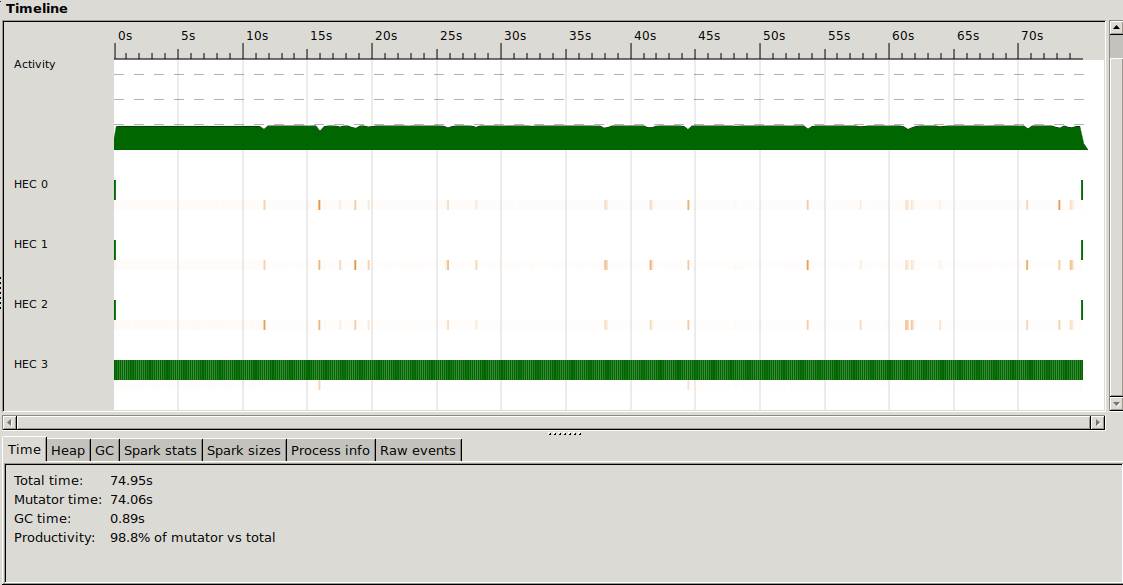
\includegraphics[width=\linewidth]{main0.png}
  \centering
  \caption{Послідовне виконання за 74.95с (ThreadScope)}
\end{figure}

\begin{figure}[H]
  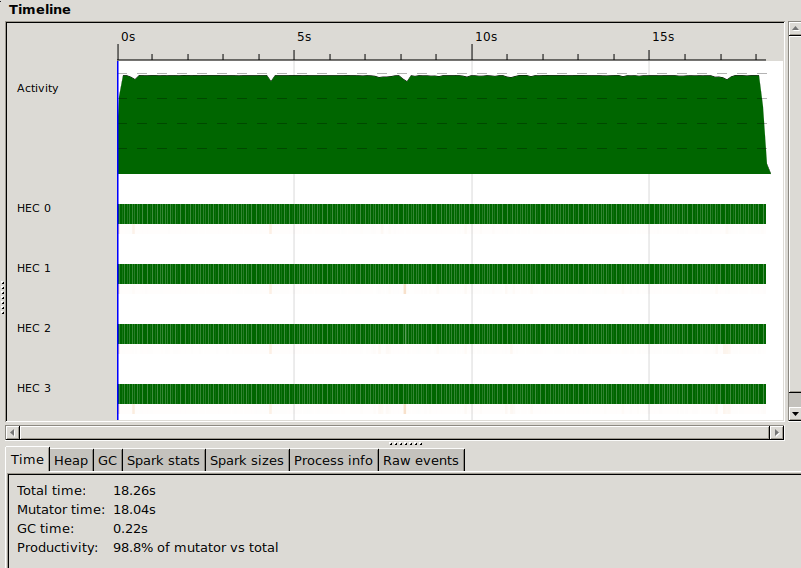
\includegraphics[width=\linewidth]{main1.png}
  \centering
  \caption{Вбудовані засоби 18.26с (ThreadScope)}
\end{figure}

\begin{figure}[H]
  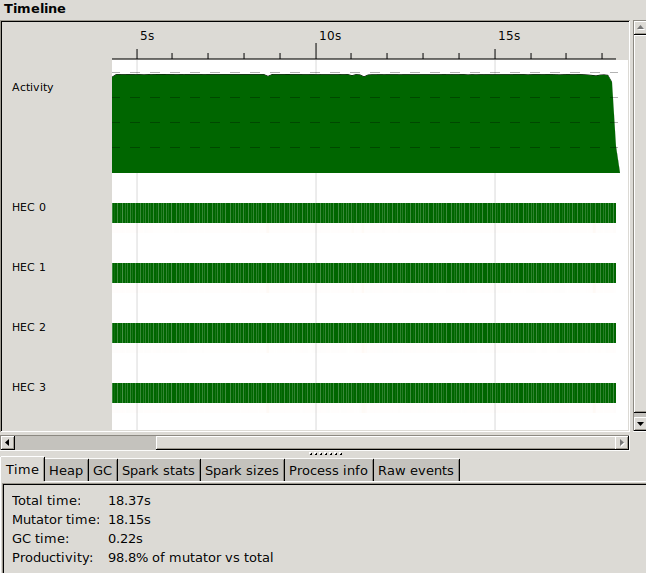
\includegraphics[width=\linewidth]{main2.png}
  \centering
  \caption{Транзакційна пам'ять за 18.37с (ThreadScope)}
\end{figure}

\begin{figure}[H]
  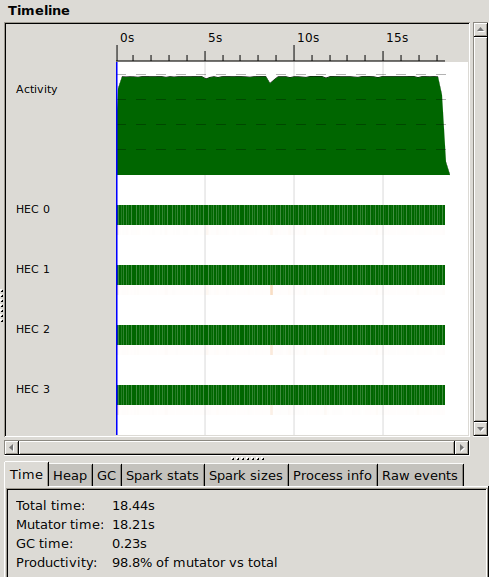
\includegraphics[width=\linewidth]{main3.png}
  \centering
  \caption{Засоби Cloud Haskell за 18.44с (ThreadScope)}
\end{figure}

При невеликій взаємодії між процесами різниця незначна. Але при використанні 
великої кількості потоків (\lstinline{nthreads} = $10^4$) CH програє за швидкістю. 
З порівняння (картинка \ref{compare10K}) можна побачити, що другий варіант (CH) потребує 
в 6 разів більше часу на сміттєзбірочні роботи(виклики GC позначено жовтими паличками). 
В той же час приріст часу для першого варіанту (STM) ледь помітно.
Якщо ми заглянемо до вихідних кодів бібліотеки, то знайдемо відповідь - сама 
бібліотека написана з використанням тих самих вбудованих примітивів та транзакційної
пам'яті. При тому, створюється набагато більше роздільних змінних 
(по декілька TVar-ів на актора проти лише двох для STM варіанту), збільшуючи накладні
витрати.\\

За результатами порівняння можна відчути, що порівняно зі стандартними засобами модель акторів має ту перевагу, що, на відміну від STM та Control.Concurrent, при роботі з нею протягом всього реферату автор не отримав жодного дедлоку. Також, модель акторів є більш органічним та зрозумілим способом конкурентного програмування.\\

Для розподіленого програмування на Гаскелі це фактично єдиний можливий на сьогодні варіант, тож й порівнювати нема з чим\footnote{Дві інші спроби - Eden та GdH не розвиваються з 2014 та 2005 років
відповідно. Прив'язки до MPI також покинуті автором з 2015. 
В свою чергу, CH активно розробляється комерційною компанією Well-Typed LLP.}. Порівняння з Erlang та Scala має сенс, але відносно скромне знання автором цих мов підштовхнуло останнього до виключення цього розділу з викладу.\\

Порівняння з C, в свою чергу, не складає великої цінності, бо невтішні для гаскелю результати такого порівняння можна легко передбачити наперед.

\begin{figure}
\hfill
\subfigure[STM за 18.88с]{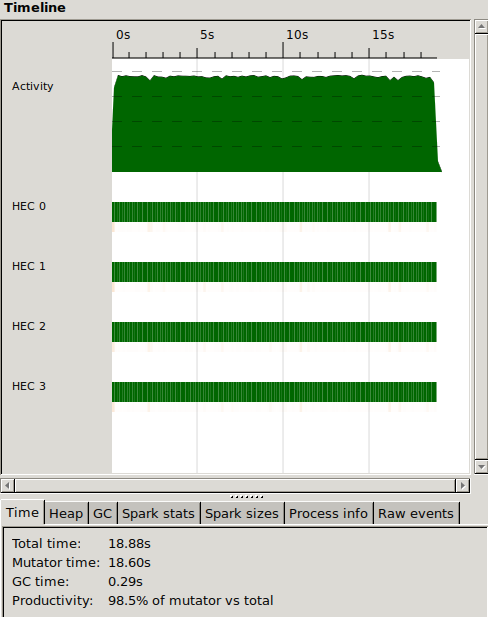
\includegraphics[width=0.45\linewidth]{main2_10K.png}}
\hfill
\subfigure[CH за 31.43с]{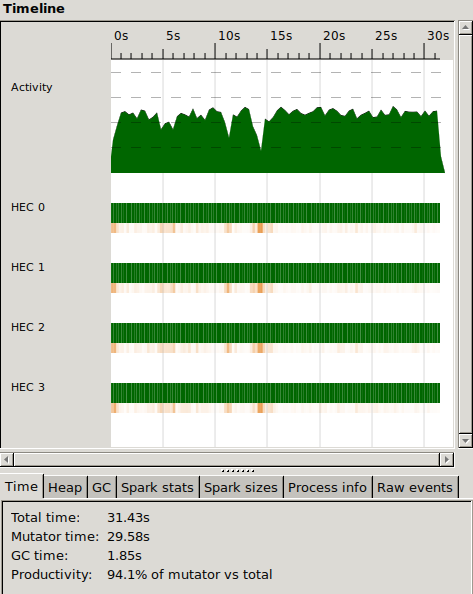
\includegraphics[width=0.45\linewidth]{main3_10K.png}}
\hfill
\caption{Порівняння транзакційної пам'яті та Cloud Haskell за \lstinline{nthreads} = $10^4$}
\label{compare10K}
\end{figure}

\section{Лічильник Армстронга}
\epigraph{One end is no end}{Карл Г'юїтт}

Лічильник Армстронга - популярна демонстраційна розподілена програма, наведена у книзі 
Д. Армстронга\cite{programmingErlang}. Програма може бути або лічильником, або терміналом доступу. Кожен лічильник зберігає свій стан. З терміналу можна керувати віддаленими лічильниками - збільшити на одиницю, отримати поточне значення, або наказати лічильникові вмерти. Головна ідея цього прикладу полягає скоріше в 
демонстрації мережевих можливостей CH. Автор використовував в якості <<кластера>> 
свій ноутбук. Обидва вони належать до локальної мережі домашнього рутера.
Ноутбук буде використовуватися в якості єдиного slave-а, стаціонарний ПК, конфігурацію
якого детально описано на початку реферату - як master.\\

\begin{lstlisting}[language=bash, caption=Конфігурація другого комп'ютера]
[nik@nixos:~]$ screenfetch 
          ::::.    ':::::     ::::'           nik@nixos
          ':::::    ':::::.  ::::'            OS: NixOS 
            :::::     '::::.:::::             Kernel: x86_64 Linux 
      .......:::::..... ::::::::                      4.9.38
     ::::::::::::::::::. ::::::    ::::.      Packages: 3920
    ::::::::::::::::::::: :::::.  .::::'      Shell: bash
           .....           ::::' :::::'       Resolution: 1366x768
          :::::            '::' :::::'        WM: XMonad
 ........:::::               ' :::::::::::.   CPU:Intel Core i5-6200U 
:::::::::::::                 :::::::::::::   4x 2.8GHz [30.0 C]
 ::::::::::: ..              :::::            RAM: 441MiB / 3848MiB
     .::::: .:::            :::::            
    .:::::  :::::          '''''    .....    
    :::::   ':::::.  ......:::::::::::::'    
     :::     ::::::. ':::::::::::::::::'     
            .:::::::: '::::::::::            
           .::::''::::.     '::::.           
          .::::'   ::::.     '::::.          
         .::::      ::::      '::::.         
\end{lstlisting}

Для успішного запуску
необхідно по-перше вимкнути фаєрвол, а по-друге ввімкнути UDP multicast, 
бо саме за цим протоколом працює пошук пірів. Перше можна зробити в
\lstinline{/etc/nixos/configuration.nix}, задавши 
\lstinline{networking.firewall.enable = false;} та \lstinline{$ sudo nixos-rebuild switch}.
Друге можна виконати як \lstinline{$ sudo ifconfig lo multicast}.\\

Для роботи визначимо простий тип команд.\\

\begin{lstlisting}{src/Armstrong.hs}
data Command = Increment
             | Get ProcessId
             | Suicide
             deriving (Typeable, Generic)

instance Binary Command
\end{lstlisting}

Функціонал терміналу доступу. Зауважте, що на кожному терміналі 2 процеси, один для користувацького вводу, інший для виводу повідомлень.\\

\begin{lstlisting}{src/Armstrong.hs}
master :: Backend -> Process ()
master backend = do
  pid <- spawnLocal logCounter
  run pid
  where
    usage = "Usage: I(ncrement) | G(et) | S(uicide)"
    
    parse i "G" = Just (Get i)
    parse _ "I" = Just Increment
    parse _ "S" = Just Suicide
    parse _  _  = Nothing

    logCounter = do
      (from, n) :: (ProcessId, Int) <- expect
      liftIO $ putStrLn $ "{" ++ show from ++ " = " ++ show n ++ "}"
      logCounter
      
    run pid = do
      slaves <- findSlaves backend
      liftIO $ putStrLn $ "[" ++ show (length slaves) ++ "] Enter message: "
      msg <- liftIO $ getLine
      case parse pid msg of
        Nothing -> do liftIO $ putStrLn usage
        Just cmd -> forM_ slaves $ flip send cmd
      run pid
\end{lstlisting}

Слейви мають бути зареєстровані як slaveController, щоб пошук findSlaves їх автоматично підібрав.\\

\begin{lstlisting}{src/Armstrong.hs}
slave :: Process ()
slave = do
  me <- getSelfPid
  register "slaveController" me
  go me (0 :: Int)
  where go me n = do
          cmd :: Command <- expect
          n' <- case cmd of
            Increment -> return (n + 1)
            Suicide -> die Suicide
            Get pid -> send pid (me, n) >> return n
          liftIO $ putStrLn $ "[" ++ show n' ++ "]"
          go me n'
\end{lstlisting}

Програму можна запустити в двох режимах.\\

\begin{lstlisting}{src/Armstrong.hs}
main :: IO ()
main = do
  args <- getArgs
  case args of
    ["master", host, port] -> do
      backend <- initializeBackend host port initRemoteTable
      node <- newLocalNode backend
      runProcess node (master backend)
    ["slave", host, port] -> do
      backend <- initializeBackend host port initRemoteTable
      node <- newLocalNode backend
      runProcess node slave
\end{lstlisting}

Нижче наведено приклад користувацької сесії. Можна відчути, що актуалізація всієї мережі створює затримку приблизно в одну секунду, тож в реальних додатках доцільно використовувати більш розумні техніки виявлення падінь, наприклад, монітори.\\

\begin{lstlisting}[language=bash, caption=Приклад використання - Мастер]
[nik@nixos:~/projects/CloudRef]$ stack exec -- Armstrong master 192.168.0.53 7000
Master started!
[1] Enter message: 
A
Usage: I(ncrement) | G(et) | S(uicide)
[1] Enter message: 
I
[1] Enter message: 
I
[1] Enter message: 
I
[1] Enter message: 
G
{pid://192.168.0.90:7000:0:8 = 3}
[1] Enter message: 
S
[0] Enter message: 
I
[0] Enter message: 
G
[1] Enter message: 
I
[1] Enter message: 
I
I[1] Enter message: 

I[1] Enter message: 

[1] Enter message: 
I
[1] Enter message: 
S
[0] Enter message:
\end{lstlisting}

На віддаленому комп'ютері бачимо такий результат:\\

\begin{lstlisting}[language=bash, caption=Приклад використання - Слейв]
[nik@nixos:~/projects/CloudRef]$ stack exec -- 
Armstrong s
[1]
[2]
[3]
[3]
Armstrong: exit-from=pid://192.168.0.90:7000:0:8

[nik@nixos:~/projects/CloudRef]$ stack exec -- 
Armstrong s
[1]
[2]
[3]
[4]
[5]
Armstrong: exit-from=pid://192.168.0.90:7000:0:8
\end{lstlisting}

\section{Філософська вечеря}

Спробуємо розв'язати класичну задачу про філософів, що обідають, з використанням 
Cloud Haskell. Імплементуємо тривіальне рішення з додатковим актором - столом.\\

Введемо синоніми типів Philosopher та Fork. Кожен філософ може або спробувати 
взяти пару виделок, або їх повернути.\\

\begin{lstlisting}{src/Philosophers.hs}
type Philosopher = String
type Fork = Int

data TableInteraction = GrabForks ProcessId (Fork, Fork)
                      | ReleaseForks (Fork, Fork)
                      deriving (Show, Eq, Typeable, Generic)

instance Binary TableInteraction  
\end{lstlisting}

\begin{lstlisting}{src/Philosophers.hs}
think :: Philosopher -> Process ()
think p = do
  say $ p ++ " is thinking"
  r <- liftIO $ randomRIO (1,100)
  liftIO $ threadDelay $ r * 100

eat :: Philosopher -> Fork -> Fork -> Process ()
eat p _ _ = do
  say $ p ++ " is eating"
  r <- liftIO $ randomRIO (1,100)
  liftIO $ threadDelay $ r * 100
\end{lstlisting}

При ініціалізації, філософ очікує, що йому скажуть про його стіл та виделки. 
Далі в циклі філософ надсилає запит виделок столові, і очікує на них. Якщо стіл
не повернув виделок, то філософ думає. Якщо виделки прийшли - він їсть та повертає 
виделки столові. Слід відмітити, що в гаскелі, як і в ерланзі, стандартний спосіб
зберігати декотрі змінні - це рекурсія.\\

\begin{lstlisting}{src/Philosophers.hs}
philosopher p = do
  (table, forks) <- expect
  me <- getSelfPid
  loop table forks me
  where
    loop table forks me = do      
      send table $ GrabForks me forks
      maybeForks <- expect
      case maybeForks of
        Nothing -> return ()
        Just (f1, f2) -> do
          eat p f1 f2
          send table $ ReleaseForks forks
      think p
      loop table forks me
\end{lstlisting}

Якщо хтось повернув виделки - додаємо їх до списку. Якщо запитав - перевіряємо їхню наявність
та видаляємо при виділенні.\\

\begin{lstlisting}{src/Philosophers.hs}
table forks = do
  interaction <- expect
  case interaction of
    ReleaseForks (f1, f2) -> table $ f1:f2:forks
    GrabForks pid fs@(f1, f2) -> do
      let (msg, forks') =
            if f1 `elem` forks && f2 `elem` forks
            then (Just fs, forks \\ [f1, f2])
            else (Nothing, forks)
      send pid msg
      table forks'
\end{lstlisting}

Створюємо 7 процесів - стіл, філософи, офіціант, який проводить наших  
філософів\footnote{На жаль, в класичному формулюванні філософів 5 і неможливо 
зберегти баланс Сили між Континентальною та Аналітичною школами} до столів та видає
їм столові прибори.\\

\begin{lstlisting}{src/Philosophers.hs}
main :: IO ()
main = do
  let philosophers =
        [ "Zizek"
        , "Sloterdijk"
        , "Chalmers"
        , "Dennett"
        , "MacIntyre" ]

  let forks = [1..5]
      forkSets = zip forks (tail . cycle $ forks)
  
  t <- liftIO createTransport
  node <- newLocalNode t initRemoteTable

  table <- forkProcess node $ table forks
  ps <- forM philosophers $  forkProcess node . philosopher

  waiter <- forkProcess node $ do
    forM_ (ps `zip` forkSets) $ \(p, fs) -> send p (table, fs)

  liftIO getLine
  closeTransport t
\end{lstlisting}

Результати 10 секундної трапези приведені в таблиці \ref{dinnerResults}.\\


\begin {table}[H]
\begin{center}
\begin{tabular}{ c|c|c } 
            & Їв          & Думав   \\ \hline
Жіжек       & 416         & 1087    \\ 
Слотердайк  & 416         & 1129    \\ 
Макінтайр   & 412         & 1099    \\ 
Чалмерс     & 440         & 1135    \\ 
Денет       & 402         & 1092    \\ 
\end{tabular}
\caption {Трапеза}
\label{dinnerResults}
\end{center}
\end {table}


\section{MapReduce}

MapReduce - це програмна модель та програмний каркас, що її реалізує, розроблені 
компанією Google для розподіленої паралельної обробки великих масивів. MapReduce 
обчислення складається з декількох маперів, які обробляють пари ключ/значення і 
генерують набір проміжних пар ключ/значення, та меншої кількості редукторів, які об'єднують 
результати обчислень з одним і тим же проміжним ключем. Цю узагальнену схему реалізує
тип MapReduce.\\

\begin{lstlisting}{src/MapReduce/MapReduce.hs}
data MapReduce k1 v1 k2 v2 v3 = MapReduce {
    mrMap    :: k1 -> v1 -> [(k2, v2)]
  , mrReduce :: k2 -> [v2] -> v3
  } deriving (Typeable)

localMapReduce :: forall k1 k2 v1 v2 v3. Ord k2 =>
                  MapReduce k1 v1 k2 v2 v3
               -> Map k1 v1
               -> Map k2 v3
localMapReduce mr = reducePerKey mr . groupByKey . mapPerKey mr

reducePerKey :: MapReduce k1 v1 k2 v2 v3 -> Map k2 [v2] -> Map k2 v3
reducePerKey mr = Map.mapWithKey (mrReduce mr)

groupByKey :: Ord k2 => [(k2, v2)] -> Map k2 [v2]
groupByKey = Map.fromListWith (++) . map (second return)

mapPerKey :: MapReduce k1 v1 k2 v2 v3 -> Map k1 v1 -> [(k2, v2)]
mapPerKey mr = concatMap (uncurry (mrMap mr)) . Map.toList
\end{lstlisting}

В нашому прикладі будемо використовувати MapReduce для підрахунку частот слів в файлі.
В дисертації Джефрі Епштейна\cite{epsteinThesis} наводиться приклад MapReduce обчислення k-середніх, 
про який авторо стверджується, що на великих наборах даних CH обігнав Apache Hadoop.\\

\begin{lstlisting}{src/MapReduce/CountWords.hs}
type Document  = String
type Word      = String
type Frequency = Int

countWords :: MapReduce FilePath Document Word Frequency Frequency
countWords = MapReduce {
    mrMap    = const (map (, 1) . words)
  , mrReduce = const sum
  }

localCountWords :: Map FilePath Document -> Map Word Frequency
localCountWords = localMapReduce countWords

countWords_ :: () -> MapReduce FilePath Document Word Frequency Frequency
countWords_ () = countWords

remotable ['countWords_]

distrCountWords :: [NodeId] -> Map FilePath Document -> Process (Map Word Frequency)
distrCountWords = distrMapReduce ($(mkClosure 'countWords_) ())
\end{lstlisting}

Розподіл роботи виконується за схемою Work-stealing за допомогою черги.\\

\begin{lstlisting}{src/MapReduce/MonoDistrMapReduce.hs}
mapperProcess :: (ProcessId, ProcessId, Closure (MapReduce String String String Int Int))
              -> Process ()
mapperProcess (master, workQueue, mrClosure) = do
    us <- getSelfPid
    mr <- unClosure mrClosure
    go us mr
  where
    go us mr = do
      -- Просимо роботи в черги
      send workQueue us
      say "Ask for work"

      -- Чекаємо на відповідь
      receiveWait
        [ match $ \(key, val) -> do
            say "Mapping..."
            send master (mrMap mr key val)
            say "Mapped!"
            go us mr
        , match $ \()         -> return ()
        ]

remotable ['mapperProcess]
\end{lstlisting}

Головний вузол виконує 2 функції - видає роботу маперам, та проводить 
підсумкову редукцію.\\

\begin{lstlisting}{src/MapReduce/MonoDistrMapReduce.hs}
distrMapReduce :: Closure (MapReduce String String String Int Int)
               -> [NodeId]
               -> Map String String
               -> Process (Map String Int)
distrMapReduce mrClosure mappers input = do
  mr     <- unClosure mrClosure
  master <- getSelfPid

  workQueue <- spawnLocal $ do
    -- Висилаємо маперам нову частину роботи
    forM_ (Map.toList input) $ \(key, val) -> do
      them <- expect
      send them (key, val)

    -- Завершимо всі mapper-и
    replicateM_ (length mappers) $ do
      them <- expect
      send them ()

  -- Запускаємо мапери
  say "Waking up mappers..."
  forM_ mappers $ \nid -> do
    spawn nid ($(mkClosure 'mapperProcess) (master, workQueue, mrClosure))

  partials <- replicateM (Map.size input) expect

  say "Reducing..."
  -- Маємо єдиний редуктор на цій ноді
  return (reducePerKey mr . groupByKey . concat $ partials)
\end{lstlisting}

Головна програма реалізує простий користувацький інтерфейс.
Використовуються стандартні мастер та слейв функції.

\begin{lstlisting}{src/MapReduce/SimpleLocalnet.hs}
main :: IO ()
main = do
  args <- getArgs

  case args of
    -- Локальне рахування слів
    "local" : "count" : files -> do
      input <- constructInput files
      print $ CountWords.localCountWords input

    -- Розподілений підрахунок слів
    "master" : host : port : "count" : files -> do
      input   <- constructInput files
      backend <- initializeBackend host port rtable
      startMaster backend $ \slaves -> do
        result <- CountWords.distrCountWords slaves input
        liftIO $ print result

    -- slave
    "slave" : host : port : [] -> do
      backend <- initializeBackend host port rtable
      startSlave backend
\end{lstlisting}

На жаль, як можна побачити з приведених нижче результатів, експеримент виявився невдалим.
Задачу підрахування частот для 7 файлів розміром 4.5 мегабайт пришвидчити не вдалося.
Можливі причини невдачі - великі накладні витрати на використання мережі на редукцію, 
помилка при проектуванні програми, відносно легкі процеси віддані маперам.

\begin{lstlisting}[language=bash, basicstyle=\ttfamily\small, caption=4 локальних та 4 віддалених мапера]
time stack exec -- MapReduce master 192.168.0.53 60000 count a b c d e f g >> /dev/null
Thu Nov 23 15:40:21 UTC 2017 pid://192.168.0.53:60000:0:8: Begin
Thu Nov 23 15:40:21 UTC 2017 pid://192.168.0.53:60000:0:8: Waking up mappers...
Thu Nov 23 15:40:21 UTC 2017 pid://192.168.0.90:5001:0:12: Ask for work
Thu Nov 23 15:40:21 UTC 2017 pid://192.168.0.90:5002:0:12: Ask for work
Thu Nov 23 15:40:21 UTC 2017 pid://192.168.0.90:5003:0:12: Ask for work
Thu Nov 23 15:40:21 UTC 2017 pid://192.168.0.90:5004:0:12: Ask for work
Thu Nov 23 15:40:21 UTC 2017 pid://192.168.0.53:60003:0:15: Ask for work
Thu Nov 23 15:40:21 UTC 2017 pid://192.168.0.53:60006:0:15: Ask for work
Thu Nov 23 15:40:21 UTC 2017 pid://192.168.0.53:60005:0:15: Ask for work
Thu Nov 23 15:40:21 UTC 2017 pid://192.168.0.53:60004:0:15: Ask for work
Thu Nov 23 15:40:23 UTC 2017 pid://192.168.0.90:5001:0:12: Mapping...
Thu Nov 23 15:40:25 UTC 2017 pid://192.168.0.90:5002:0:12: Mapping...
Thu Nov 23 15:40:26 UTC 2017 pid://192.168.0.90:5003:0:12: Mapping...
Thu Nov 23 15:40:27 UTC 2017 pid://192.168.0.90:5004:0:12: Mapping...
Thu Nov 23 15:40:28 UTC 2017 pid://192.168.0.53:60003:0:15: Mapping...
Thu Nov 23 15:40:28 UTC 2017 pid://192.168.0.53:60006:0:15: Mapping...
Thu Nov 23 15:40:28 UTC 2017 pid://192.168.0.90:5001:0:12: Mapped!
Thu Nov 23 15:40:28 UTC 2017 pid://192.168.0.90:5001:0:12: Ask for work
Thu Nov 23 15:40:28 UTC 2017 pid://192.168.0.53:60005:0:15: Mapping...
Thu Nov 23 15:40:29 UTC 2017 pid://192.168.0.53:60003:0:15: Mapped!
Thu Nov 23 15:40:29 UTC 2017 pid://192.168.0.53:60003:0:15: Ask for work
Thu Nov 23 15:40:30 UTC 2017 pid://192.168.0.53:60006:0:15: Mapped!
Thu Nov 23 15:40:30 UTC 2017 pid://192.168.0.53:60006:0:15: Ask for work
Thu Nov 23 15:40:30 UTC 2017 pid://192.168.0.53:60005:0:15: Mapped!
Thu Nov 23 15:40:30 UTC 2017 pid://192.168.0.53:60005:0:15: Ask for work
Thu Nov 23 15:40:31 UTC 2017 pid://192.168.0.90:5002:0:12: Mapped!
Thu Nov 23 15:40:31 UTC 2017 pid://192.168.0.90:5002:0:12: Ask for work
Thu Nov 23 15:40:32 UTC 2017 pid://192.168.0.90:5003:0:12: Mapped!
Thu Nov 23 15:40:32 UTC 2017 pid://192.168.0.90:5003:0:12: Ask for work
Thu Nov 23 15:40:32 UTC 2017 pid://192.168.0.90:5004:0:12: Mapped!
Thu Nov 23 15:40:32 UTC 2017 pid://192.168.0.90:5004:0:12: Ask for work
Thu Nov 23 15:40:36 UTC 2017 pid://192.168.0.53:60000:0:8: Reducing...

real    0m43.772s
user    0m36.316s
sys     0m1.887s
\end{lstlisting}

\begin{lstlisting}[language=bash, basicstyle=\ttfamily\small, caption=4 локальних мапери]
time stack exec -- MapReduce master 192.168.0.53 60000 count a b c d e f g >> /dev/null
Thu Nov 23 15:44:21 UTC 2017 pid://192.168.0.53:60000:0:8: Begin
Thu Nov 23 15:44:21 UTC 2017 pid://192.168.0.53:60000:0:8: Waking up mappers...
Thu Nov 23 15:44:21 UTC 2017 pid://192.168.0.53:60003:0:16: Ask for work
Thu Nov 23 15:44:21 UTC 2017 pid://192.168.0.53:60005:0:16: Ask for work
Thu Nov 23 15:44:21 UTC 2017 pid://192.168.0.53:60004:0:16: Ask for work
Thu Nov 23 15:44:21 UTC 2017 pid://192.168.0.53:60006:0:16: Ask for work
Thu Nov 23 15:44:23 UTC 2017 pid://192.168.0.53:60003:0:16: Mapping...
Thu Nov 23 15:44:24 UTC 2017 pid://192.168.0.53:60005:0:16: Mapping...
Thu Nov 23 15:44:24 UTC 2017 pid://192.168.0.53:60004:0:16: Mapping...
Thu Nov 23 15:44:25 UTC 2017 pid://192.168.0.53:60006:0:16: Mapping...
Thu Nov 23 15:44:25 UTC 2017 pid://192.168.0.53:60003:0:16: Mapped!
Thu Nov 23 15:44:25 UTC 2017 pid://192.168.0.53:60003:0:16: Ask for work
Thu Nov 23 15:44:26 UTC 2017 pid://192.168.0.53:60005:0:16: Mapped!
Thu Nov 23 15:44:26 UTC 2017 pid://192.168.0.53:60005:0:16: Ask for work
Thu Nov 23 15:44:26 UTC 2017 pid://192.168.0.53:60004:0:16: Mapped!
Thu Nov 23 15:44:26 UTC 2017 pid://192.168.0.53:60004:0:16: Ask for work
Thu Nov 23 15:44:27 UTC 2017 pid://192.168.0.53:60006:0:16: Mapped!
Thu Nov 23 15:44:27 UTC 2017 pid://192.168.0.53:60006:0:16: Ask for work
Thu Nov 23 15:44:28 UTC 2017 pid://192.168.0.53:60003:0:16: Mapping...
Thu Nov 23 15:44:30 UTC 2017 pid://192.168.0.53:60003:0:16: Mapped!
Thu Nov 23 15:44:30 UTC 2017 pid://192.168.0.53:60003:0:16: Ask for work
Thu Nov 23 15:44:29 UTC 2017 pid://192.168.0.53:60005:0:16: Mapping...
Thu Nov 23 15:44:30 UTC 2017 pid://192.168.0.53:60005:0:16: Mapped!
Thu Nov 23 15:44:30 UTC 2017 pid://192.168.0.53:60005:0:16: Ask for work
Thu Nov 23 15:44:29 UTC 2017 pid://192.168.0.53:60004:0:16: Mapping...
Thu Nov 23 15:44:31 UTC 2017 pid://192.168.0.53:60004:0:16: Mapped!
Thu Nov 23 15:44:31 UTC 2017 pid://192.168.0.53:60004:0:16: Ask for work
Thu Nov 23 15:44:35 UTC 2017 pid://192.168.0.53:60000:0:8: Reducing...

real    0m40.234s
user    0m35.479s
sys     0m1.929s
\end{lstlisting}

\begin{lstlisting}[language=bash, basicstyle=\ttfamily\small, caption=Послідовний варіант]
time stack exec -- MapReduce local count a b c d d e f g >> /dev/null

real    0m34.580s
user    0m33.182s
sys     0m1.448s
\end{lstlisting}

\section{Розподілене KV-сховище}

Даний приклад націлено не на демонстрацію пришвидшення паралельних обчислень, а на 
ілюстрацію того, як можна зробити деякі важливі обчислення відказостійкими. Нехай є
декілька комп'ютерів (для простоти промоделюємо їх як окремі процеси). Ми хочемо зберігати 
на кожному декотру інформацію, а також мати можливість її зчитувати. Для простоти
будемо зберігати її лише в оперативній пам'яті. Хоча тут маємо цілком шкільний приклад,
розподілені сховища даних є одними з найважливіших застосувань акторних обчислень.\\

Створимо необхідні типи.\\

\begin{lstlisting}{src/KV/Request.hs}
type Key   = String
type Value = String

data Request = GET Key (SendPort (Maybe Value))
             | SET Key Value
             deriving (Typeable,Generic)

instance Binary Request
\end{lstlisting}

Функція, яку буде запущено на віддалених нодах. SET запроси обробляються напряму, 
GET - з використанням каналу.\\

\begin{lstlisting}{src/KV/Worker.hs}
worker :: Process ()
worker = loop Map.empty
    where
        loop db = do
            r <- expect :: Process Request
            case r of
              SET k v -> do
                let newdb = Map.insert k v db
                loop newdb
              GET k s -> do
                let mval = Map.lookup k db
                sendChan s mval
                loop db
                    
remotable ['worker]
\end{lstlisting}

Функції для мережевої взаємодії:

\begin{lstlisting}{src/KV/Database.hs}
set :: Database -> Key -> Value -> Process ()
set db k v = send db (SET k v)

get :: Database -> Key -> Process (Maybe Value)
get db k = do
    (s,r) <- newChan 
    let req = GET k s 
    send db (GET k s)
    receiveChan r 
\end{lstlisting}

Мастер процес, тобто база даних, працює так. Спочатку від'єднується паралельний 
процес, який моніторить кількість живих рабів (доки є хоча б один живий), 
а якщо хтось від'єднався - сповіщає користувача. Зауважимо, що для роботи
треба мінімум 2 вузли. Живі раби зберігаються в транзакційній змінній.\\

\begin{lstlisting}{src/KV/Database.hs}
database :: [NodeId] -> Process ()
database nodes = do
    ps <- mapM (\n -> spawn n $(mkStaticClosure 'worker)) nodes

    tps <- liftIO $ newTVarIO (pairs ps)
    spawnLocal $ do 
      mapM_ monitor ps 
      whileM_  (do
                   pids <- liftIO $ atomically $ readTVar tps
                   return $ length pids > 0
               )$
        receiveWait 
        [ match $ \(ProcessMonitorNotification ref deadpid reason) -> do
                    liftIO $ atomically $ modifyTVar' tps $ map (delete deadpid)
                    say $ printf "process %s died: %s" (show deadpid) (show reason)
        ]                      
                   
    forever $ do
      r <- expect :: Process Request
      ps' <- liftIO $ atomically $ readTVar tps
      case r of
        GET k s-> mapM_ (\p -> send p r) (npid k ps') 
        SET k v -> mapM_ (\p -> send p r) (npid k ps') 
    where
        pairs [] = []
        pairs [x] = []
        pairs (x:y:xs) = [x,y] : pairs xs
        npid k ps = ps !! (ord (head k) `mod` length ps)
\end{lstlisting}

Проста точка входу дозволяє вводити команди. Функція distribMain обробляє аргументи
безпосередньо програми за допомогою нудного boilerplate коду, який немає сенсу приводити.
Для спрощення використовуються стандартні функції слейвів та мастерів.\\

\begin{lstlisting}{src/KV/Main.hs}
main = distribMain master rcdata

master :: [NodeId] -> Process ()
master peers = do
  db <- createDB peers
  liftIO $ print peers
  set db "a" "1"
  forever $ do
    liftIO $ putStrLn "ENTER COMMAND:"
    cmd <- liftIO getLine
    case words cmd of
      ["SET", k, v] -> do
        set db k v
      ["GET", k] -> do
        v <- get db k
        liftIO $ putStrLn $ "response: " ++ show v
      _ -> liftIO $ putStrLn $ "usage: SET k v | GET k"

  return ()
\end{lstlisting}

Для демонстрації запустимо декілька слейвів \lstinline{stack exec -- KV slave 44447 &} та запустимо 
мастер-термінал. Потім спробуємо зупинити декілька процесів, і перевірити працездатність та цілісність 
сховища. Можна також погратися з декількома точками доступу (Універсальні слейви не будуть змішувати дані різних мастерів).\\

\begin{lstlisting}[language=bash, caption=Приклад сесії]
$ stack exec -- KV master
[nid://127.0.0.1:44447:0,nid://127.0.0.1:44446:0,
nid://127.0.0.1:44427:0,nid://127.0.0.1:44448:0]
ENTER COMMAND:
GET a
response: Just "1"
ENTER COMMAND:
GET b
response: Nothing
ENTER COMMAND:
SET a 12
ENTER COMMAND:
GET a
response: Just "12"
ENTER COMMAND:
Wed Nov 22 19:56:37 UTC 2017 pid://127.0.0.1:44444:0:10: process
    pid://127.0.0.1:44446:0:10 died: DiedDisconnect
GET a
response: Just "12"
ENTER COMMAND:
SET a 5
ENTER COMMAND:
GET a
response: Just "5"
ENTER COMMAND:

\end{lstlisting}


\section{Допоміжна довідка}

\subsubsection*{Лямбда числення}

Більш розгорнуте викладення можна знайти, наприклад у\cite{lambdaMoskvin}.\\

Синтаксис лямбда числення задається наступною граматикою:
\begin{lstlisting}[caption={Синтаксис простого безтипового лямбда числення}]
Нескінченна перелічувана множина змінних:
V ::= x | y | x1 | ... 

Термом є змінна, абстракція, або аплікація:
M, N ::= V
     | (\V -> M)
     | (M N)
\end{lstlisting}

При цьому, абстракція є правоасоціативною, аплікація - лівоасоциативною.\\

Множина вільних змінних \lstinline{FV(M)} терму \lstinline{N} задається рекурентно:\\
\begin{lstlisting}[caption={Вільні змінні}]
FV(x) = {x}
FV(\x -> P) = FV(M) \ {x}
FV(P Q) = FV(P) ∪ FV (Q)
\end{lstlisting}

Вільна змінна не зв'язана жодною лямбда абстракцією, наприклад в термі \lstinline{(\f -> (\x -> f x))} 
всі змінні зв'язані, але з точки зору його внутрішнього терму \lstinline{(\x -> f x)} змінна y є вільною.\\

Функція (тобто $\lambda$-терм) є замкненою, якщо множина її вільних змінних є пустою.

Підстановкою терма замість змінної в термі визначають так:
\begin{lstlisting}[caption={Вільні змінні}]
x[x := N] = N
y[x := N] = y
(P Q)[x := N] = P[x := N] Q[x := N]
(\x -> P)[x := N] = \x -> P
(\y -> P)[x := N] = \y -> P[x := N]
\end{lstlisting}

Підстановка вважається правильною, якщо жодна вільна змінна не стає зв'язаною, зв'язана - вільною.\\

Відношенням бета-редукції \lstinline{=>} називають таке найменше відношення на множині $\lambda$-термів, що \\
\begin{itemize}
    \item \lstinline{(\x -> P) Q => P[x:=Q]}
    \item Якщо \lstinline{P => P'}, то \lstinline{\x -> P => \x -> P'}
    \item Якщо \lstinline{P => P'}, то \lstinline{P Q => P' Q}
    \item Якщо \lstinline{P => P'}, то \lstinline{Q P => Q P'}
\end{itemize}

Ліву частину редукції називають редексом, праву - згортком. Якщо терм не є редексом, 
то кажуть, що він знаходиться у нормальній формі.\\

Багатошаговою бета-редукцією \lstinline{=>>} називають транзитивно-рефлексивне замикання \lstinline{=>}\\

Бета-еквівалентністю називають транзитивно-рефлексивно-симетричне замикання \lstinline{=>}\\

\label{systemFC}
\subsubsection*{System FC}

Синтаксис Гаскеля зводиться до синтаксису System FC\cite{systemFC} - формальної системи поліморфного лямбда числення, 
яка розширює System F свідками приведення (Coercion).\\

Нижче приведено визначення виразу мови GHC Core, взяте з репозиторію вихідого коду GHC\cite{coreSource}.\\

\begin{lstlisting}{CoreSyn.hs}
data Expr b
  = Var   Id
  | Lit   Literal
  | App   (Expr b) (Arg b)
  | Lam   b (Expr b)
  | Let   (Bind b) (Expr b)
  | Case  (Expr b) b Type [Alt b]
  | Cast  (Expr b) Coercion
  | Tick  (Tickish Id) (Expr b)
  | Type  Type
  | Coercion Coercion
  deriving Data
\end{lstlisting}


\subsubsection*{Замикання}
Замиканням відношення $R$ відносно властивості $P$ називають таке мінімальне $R^{*}$, що $R \subset R^{*}$, 
та для будь якої пари $(x,y) \in R^{*}$ виконується $P(x,y)$. Під замиканням функції у функціональному 
програмуванні розуміють саму цю функцію разом з її оточенням, яке складається з її вільних змінних. 
Наприклад, замиканням функції \lstinline{\x -> (x z) (y x)} буде пара \lstinline{<(\x -> (x z) (y x)), [y; z]>}.\\

\subsubsection*{Лінива семантика}
Call-by-need семантика означає, що редуціюються лише ті терми, які потрібно, а не всі, на які вказав 
програміст. Продемонструємо це у GHCi\\

\begin{lstlisting}[caption={Ліниві обчислення}]
λ> :set +s
λ> fac n = product [1..n]
(0.00 secs, 0 bytes)
λ> xs = replicate 10000 (fac 25000)
(0.00 secs, 0 bytes)
λ> length xs
10000
(0.01 secs, 1,052,640 bytes)
λ> fac 25000 `mod` 2
0
(1.06 secs, 597,515,792 bytes)
λ> sum xs `mod` 2
0
(1.93 secs, 1,010,760,824 bytes)
\end{lstlisting}

Таким чином, факторіал 25000! не вираховується тисячу разів, суттєво вкорочуючи час виконання програми. 
Зауважте також, що всі операції виконуються над необмеженим типом Integral, втрати даних через 
переповнення не виходить (на відміну від типу Int).\\

Втім, гаскель має спеціальні засоби для вказання на строгий порядок редукцій.\\

\subsubsection*{Переписування графів}
Гаскель є системою лінивого переписування графів. Це означає, що кожну програму можна представити у 
вигляді графу, вузлами якого є санки(редекси), висячими вершинами - значення в нормальній формі. На 
кожному шазі виконання програми цей граф зменьшується (редуціюється). Пи цьому, синтаксично однакові 
вирази відображаються в єдиний вузол графу. Приклад редукції наведено у Рис. \ref{reduction1} на 
сторінці \pageref{reduction1}.\\

\begin{figure}
\centering

\begin{tikzpicture}

\node[shape=circle,draw=black] (A1) at (0,0) {add};
\node[shape=circle,draw=black] (M) at (-1,-1) {mul};
\node[shape=circle,draw=black] (A2) at (1,-2) {add};

\node[shape=rectangle,draw=black] (N3) at (-2,-2) {3};
\node[shape=rectangle,draw=black] (N1) at (2,-3) {1};
\node[shape=rectangle,draw=black] (N2) at (0,-3) {2};

\path [->] (A1) edge node[left] {} (M);
\path [->] (A1) edge node[left] {} (A2);
\path [->] (M) edge node[left] {} (A2);
\path [->] (M) edge node[left] {} (N3);
\path [->] (A2) edge node[left] {} (N1);
\path [->] (A2) edge node[left] {} (N2);

\end{tikzpicture}

\vspace{20mm}

\begin{tikzpicture}

\node[shape=circle,draw=black] (A1) at (0,0) {add};
\node[shape=circle,draw=black] (M) at (-1,-1) {mul};
\node[shape=rectangle,draw=black] (A2) at (1,-2) {3};

\node[shape=rectangle,draw=black] (N3) at (-2,-2) {3};

\path [->] (A1) edge node[left] {} (M);
\path [->] (A1) edge node[left] {} (A2);
\path [->] (M) edge node[left] {} (A2);
\path [->] (M) edge node[left] {} (N3);

\end{tikzpicture}

\vspace{20mm}

\begin{tikzpicture}

\node[shape=circle,draw=black] (A1) at (0,0) {add};
\node[shape=rectangle,draw=black] (M) at (-1,-1) {9};
\node[shape=rectangle,draw=black] (A2) at (1,-2) {3};

\path [->] (A1) edge node[left] {} (M);
\path [->] (A1) edge node[left] {} (A2);

\end{tikzpicture}

\vspace{20mm}

\begin{tikzpicture}

\node[shape=rectangle,draw=black] (A1) at (0,0) {27};

\end{tikzpicture}

\vspace{20mm}

\caption{Редукція терму 
\lstinline{(add (mul 3 (add 1 2)) (add 1 2))}
} 
\label{reduction1}
\end{figure}



\section{Висновок}
%Чому Ви рекомендуєте (не рекомендуєте) використання цієї технології

За результатом роботи автор може сформувати відносно суб'єктивний список приємностей та неприємностей, які він примітив в розглянутої технології.\\

Приємності:
\begin{itemize}
    \item Всі переваги Гаскеля як мови, які довго перелічувати
    \item Невеликі та порівняно зрозумілі\footnote{Звісно що з Erlang OTP та MPI} вихідні коди
    \item Чудове теоретичне підгрунтя
    \item Документація
    \item Використовується в продакшн\footnote{Це велика рідкість для Haskell бібліотек} (iohk.io та ін.)
\end{itemize}

Неприємності:
\begin{itemize}
    \item Швидкодія Гаскелю
    \item Мала популярність
    \item Невелика кількість навчальних матеріалів
\end{itemize}

\newpage

\printbibliography[title={Перелік посилань}]

\end{document}
